\chapter{Классификация гамма-всплесков, зарегистрированных в эксперименте Конус-Винд}\label{KW_GRB_classification}

\section{Введение}
Первым свидетельством наличия двух классов всплесков было обнаружение их бимодального 
распределения по длительности~\citep{Mazets_1981_part_1,Norris_1984,Kouveliotou_1993,Aptekar_1998}. 
В работе \citep{Kouveliotou_1993} были введены две меры длительности $T_{50}$ и $T_{90}$, 
которые соответствуют временам накопления 50\% и 90\% от суммарного числа отсчётов 
всплеска (интервалы от 25\% до 75\% и от 5\% до 95\% отсчётов, соответственно), 
и определена граница между длинными и короткими всплесками $T_{90}=2$~с 
на основе локального минимума бимодального распределения. 
В работе \citep{McBreen_1994} обсуждается, что распределение всплесков по 
длительности $T_{90}$ хорошо описывается суммой двух логнормальных компонент. 
Более детальный анализ распределения по $T_{90}$ всплесков из третьего каталога 
эксперимента BATSE~\citep{Horvath_2002} показал, что распределение 
хорошо аппроксимируется тремя логнормальными компонентами. 
Третья компонента располагалась между короткими и длинными всплесками, 
что свидетельствовало о наличие третьего класса всплесков с промежуточной длительностью.
Доля промежуточных всплесков составила 6\%. 

Систематические ошибки величин $T_{50}$ и $T_{90}$, которые искажают наблюдаемое 
распределение всплесков, были рассмотрены в работе~\citep{Norris_and_Bonnel_2006ApJ} 
на примере всплесков, зарегистрированных в эксперименте \textit{CGRO}-BATSE~\citep{Fishman_1992NASCP3137}. 
Было показано, что как минимум четыре фактора влияют на измеренное значение длительности 
всплеска и размывают границы между классами коротких и длинных всплесков: 
(1)~различие в отношении сигнал-шум (S/N) между самым интенсивным и самым слабым 
всплеском  при условии, что эти всплески не отличаются по другим параметрам, 
приводит к различию их длительностей $T_{90}$ в $\sim 2$~раза~\citep{Bonnell_1997}; 
(2)~длительность космологически удалённых длинных всплесков (с красными смещениями источников 
$z \sim 2 \textrm{--}10$) увеличивается в 2--5 раз по сравнению со всплесками, 
пришедшими с $z=1$, в это же время поправка длительности 
для коротких всплесков не превышает двух раз, так как их источники в основном 
расположены на $z<1$ (этот фактор увеличивает обособленность распределений 
коротких и длинных всплесков); (3)~эффект зависимости длительности отдельных импульсов 
всплесков от энергии $\propto E^{-0.35}$~\citep{Fenimore_1995}, а так же модификация 
спектра за счёт космологического расширения приводит к зависимости длительности 
всплеска от энергетического диапазона наблюдений; (4)~распределение по длительностям 
обрезано со стороны коротких всплесков вследствие наблюдательной селекции триггерного 
алгоритма. 

Кроме $T_{50}$ и $T_{90}$ была предложена и другая мера длительности~--- время 
эмиссии~\citep{Mitrofanov_1999}, которая вычисляется как суммарная длительность 
бинов временной истории, в которых интенсивность излучения превышает заданный 
уровень от пиковой интенсивности. Этот уровень задается таким образом, чтобы 
суммарное число отсчетов в бинах составляло заданную долю от общего числа отсчётов 
всплеска (использовались уровни 30\% и 50\%, соответствующие меры длительности 
были обозначены $\tau_{30}$ и $\tau_{50}$). Было показано, что данная мера 
длительности гораздо менее чувствительна и к отношению сигнал-шум и к количеству 
импульсов во всплеске, разделенных значительным промежутком фона, так как этот 
промежуток не входит, по определению, в определяемое время эмиссии. Ясно, однако, 
что эта мера чувствительна к временному разрешению. Распределения всплесков 
по $\tau_{30}$ и $\tau_{50}$  также являются бимодальными. Эти меры длительности 
не получили широкого распространения, поэтому классификация всплесков 
на их основе в данной работе не рассматривается. 

Короткие и длинные всплески, в среднем, отличаются жёсткостью спектра.
В работе \citep{Kouveliotou_1993} было обнаружено, что короткие всплески BATSE, в 
среднем, имеют большую жёсткость ($\rmn{HR}_{32}$), чем длинные, где $\rmn{HR}_{32}$ определялась 
как отношение числа отсчетов, накопленных за $T_{90}$ в энергетических 
диапазонах 100--300~кэВ и 50--100~кэВ (диапазоны 3 и 2) эксперимента \textit{CGRO}-BATSE. 
Однако, в последующих работах было отмечено, что жёсткость не является обязательной чертой 
коротких всплесков~\citep[см., например,][]{Sakamoto_2006_proc, Norris_and_Bonnel_2006ApJ}. 

На основе распределения на плоскости жёсткость-длительность также был обнаружен 
третий класс всплесков ~\citep{Mukherjee_1998, Hakkila_2000}. Анализ влияния 
систематических эффектов на наличие третьего класса всплесков был проведён 
в~\citep{Hakkila_2003}. Авторы показали, что третий класс всплесков не является 
физическим и может являться следствием селекции триггерного алгоритма. Также было 
показано, что сам по себе эффект зависимости длительности от яркости 
всплеска~\citep{Bonnell_1997} не может привести к появлению третьего класса всплесков. 
Однако, в последующей работе~\citep{Horvath_2006} были приведены доводы в пользу 
реальности третьего класса всплесков и исследовалось количество и значимость 
классов всплесков на основе параметров распределения на плоскости 
$\log T_{90}$--$\log \rmn{HR}_{32}$ для 1956 всплесков, зарегистрированных 
в эксперименте BATSE. При этом распределение аппроксимировалось 
суммой двумерных нормальных распределений. Было установлено, что распределение 
наилучшим образом описывается тремя компонентами (классами). При этом доля всплесков 
из класса с промежуточной длительностью составляет 10--15\%. Также было показано, что поправка набора 
всплесков на селекцию триггерного алгоритма сохраняет полученное разделение на классы. 
Аналогичный метод был применен к 222 всплескам \textit{Swift}-BAT~\citep{Horvath_2010}, 
при этом также было обнаружено три класса всплесков. При этом доля промежуточного 
класса всплесков составила~30\%.

Помимо жесткости и длительности, еще одним параметром для классификации всплесков 
может служить спектральная задержка. Этот параметр характеризует запаздывание 
излучения в более мягком диапазоне по отношению к излучению в более жестком диапазоне. 
Значение задержки ($\tau_\rmn{lag}$) соответствует положению  максимума 
кросскорреляционной функции временных историй в двух энергетических диапазонах~\citep{Norris_2000}. 
Анализ спектральных задержек коротких всплесков BATSE и \textit{Swift}-BAT показал, 
что они распределены вблизи нуля с разбросом 
порядка 25~мс \citep{Norris_and_Bonnel_2006ApJ, Norris_2011ApJ}. В то же время длинные 
всплески могут иметь значительные задержки. Идея о том, что различие спектральных 
задержек длинных и коротких всплесков отражает различие физических свойств источников 
всплесков, была выдвинута в работе~\citep{Gehrels_2006_Nature}.

%Существует несколько моделей, объясняющих появление спектральной задержки. 
%В работе~\citep{Ioka_and_Nakamura_2001} появление задержки объясняется, тем что 
%узкий джет наблюдается под разными углами для разных всплесков. Большая задержка 
%соответствует большему углу наблюдения относительно оси джета. 
%Авторы работы~\citep{Schaefer_2004_lag} считают, что спектральная задержка в 
%каждом импульсе всплеска характеризует время потери энергии излучающими частицами.

После начала эры многоволновых наблюдений гамма-всплесков стало возможным 
классифицировать всплески на основании параметров послесвечений и родительских галактик. 
В работах~\citep{Zhang_2006, Zhang_2007, Zhang_2009} была предложена схема классификации всплесков, 
основанная на этих параметрах, на физические типы: I и~II. Считается, что всплески типа~I, 
генерируются при слиянии компактных объектов, а всплески типа~II образуются 
при коллапсе молодых массивных звёзд. В работе~\citep{Zhang_2009} было показано, 
что всплески типа II на плоскости жёсткость-длительность располагаются в области 
длинных/мягких всплесков, при этом всплески типа~I~--- в области коротких/жестких событий. 
Авторы также отмечают, что всплески типа I обладают незначительной спектральной задержкой.

Неоднозначность соответствия коротких всплесков и всплесков типа~I связана, в том числе, с 
существованием коротких гамма-всплесков, сопровождающихся слабым сравнительно мягким 
излучением в гамма-диапазоне, длящимся десятки секунд после начального короткого импульса. 
Это явление получило название продленного излучения (EE).
Впервые этот класс всплесков был обнаружен в данных BATSE~\citep{Burenin_2000AstL} и 
Конус~\citep{Mazets_2002astro_ph}. В работе~\cite{Frederiks_2004ASPC} 
было обнаружено 11 всплесков с продлённым излучением среди 125 коротких гамма-всплесков KW. 
Для оставшихся всплесков был обнаружен избыток излучения на интервале 5--100~с в сумме временных 
профилей с вычтенным фоном. Такой же избыток был выявлен в данных 
BATSE~\citep{Lazzati_2001AandA, Connaughton_2002ApJ}, \textit{BeppoSAX}-GRBM~\citep{Montanari_2005ApJ} и 
\textit{INTEGRAL}-SPI-ACS~\citep{Minaev_2010AstL}. 
%написать про всплески с EE на BAT и GBM
Основную сложность представляет разделение коротких всплесков с EE 
и длинных всплесков. Авторы работы~\citep{Norris_and_Bonnel_2006ApJ} использовали визуальные признаки 
для выделения коротких всплесков с продлённым излучением: длительность начального 
импульса $T_{90}<2$~с, отсутствие заметной спектральной эволюции в начальном 
импульсе и EE. Авторы обнаружили в данных BATSE 8 всплесков, 
удовлетворяющих этим критериям, и показали, что их спектральные задержки близки к нулю. 
Также в работе отмечается наличие у некоторых всплесков интервала с практически нулевой интенсивностью излучения 
между начальным импульсом и продлённым излучением. Сравнение интенсивностей продлённого 
излучения для этих 8 всплесков и интенсивности излучения, обнаруженного в 
суммарном временном профиле в работе~\citep{Lazzati_2001AandA}, показывает, 
что динамический диапазон интенсивности продлённого излучения составляет $\sim 10^4$, 
так же как и динамический диапазон отношения интенсивности начального импульса и продлённого излучения.
В работе~\citep{Norris_2010ApJ} на основе 12 всплесков с продлённым излучением, зарегистрированных 
\textit{Swift}-BAT, был оценен физический порог отношения интенсивностей продлённого излучения 
и начального пика как единицы $\times 10^3$ и было показано, что для начальных импульсов 
всплесков без продлённого излучения характерны в $\sim 2\textrm{--}3$ раза меньшие длительности
 по сравнению с всплесками с EE, также всплески без продлённого излучения 
имеют меньшее число пиков в начальном импульсе.

Различие природы источников коротких гамма-всплесков с продлённым излучением и 
без него в настоящее время не подтверждено. В работе~\citep{Troja_2008MNRAS} 
было установлено, что смещения относительно центра родительской галактики 
коротких всплесков с продлённым излучением в среднем меньше, чем для всплесков без него: 
единицы и десятки килопарсек, соответственно. 
Исследование~\citep{Fong_2010ApJ} с использованием данных наблюдений 
телескопа \textit{Hubble Space Telescope} опровергло этот результат.

В данной главе анализируются временные истории всплесков, зарегистрированных в 
эксперименте Конус-Винд. Всплески классифицируются на основе длительности, жесткости и 
спектральной задержки, и определяется набор коротких всплесков для дальнейшей локализации и спектрального анализа. 
При этом обсуждается принадлежность исследуемых всплесков к типам~I и~II. 
В разделе~\ref{sec:GRB_sample} приводится описание использованного набора всплесков. 
В разделе~\ref{sec:Durations} рассматривается распределение всплесков по длительности, 
определяется граница между длинными и короткими всплесками на основе 
длительности $T_{50}$ и определяется итоговый набор коротких всплесков. 
В разделе~\ref{sec:Hardness} рассматриваются жесткости всплесков и производится 
классификация всплесков на основе соотношения жёсткость-длительность. 
В разделе~\ref{sec:Lags} анализируются спектральные задержки коротких всплесков. 
Сравнение классификации на физические типы~I и~II и классификации на основе жесткости, 
длительности и спектральной задержки приведено в разделе~\ref{sec:Phys_Classification}. 
Обобщение и обсуждение результатов приведено в разделе~\ref{sec:Conclision}.  

\section{Набор всплесков}\label{sec:GRB_sample}
За период с ноября 1994~г. по декабрь 2010~г. KW зарегистрировал 2008 гамма-всплесков 
в триггерном режиме. Среди них 69 всплесков содержат сбои, представляющие собой 
промежутки в данных во время всплеска, или значительные флуктуации фона, 
накладывающиеся на всплеск. Всего 1939 всплесков без сбоев.

Для вычисления параметров временных историй использовалась 
сшивка фоновой и триггерной записи. Длительность всплесков, у которых значительная 
часть события лежит в бине фоновой записи, предшествующем триггерной записи, может быть 
искажена из-за низкого разрешения фоновой записи. Из дальнейшего рассмотрения 
было исключено 105 таких событий. Таким образом, для анализа использовались временные 
истории 1834 гамма-всплеска. 

\section{Длительности}\label{sec:Durations}
Для вычисления длительностей мы использовали сумму временных историй всплеска 
в энергетических диапазонах G2 и G3. Такой выбор обоснован тем, что  пиковая 
энергия $E F_{E}$ спектра ($E_\rmn{p}$) абсолютного большинства всплесков лежит в 
диапазоне $E_\rmn{p}>80$~кэВ, и, следовательно, отсчёты, соответствующие основному энерговыделению 
во всплеске, регистрируются в диапазонах G2 и G3. Фон в G2 и G3 стабилен на более 
длительных интервалах времени, чем в G1. Это позволяет с гораздо меньшей вероятностью 
неверно определять начало и конец всплеска из-за флуктуаций фона. Также в диапазон G1 
может попадать начало рентгеновского послесвечения, учёт которого исказит 
длительность начального импульса всплеска.

Уровни фона для вычисления длительностей определялись по методике, описанной в 
разделе~\ref{sec:Bg_rate} Главы~\ref{KW_description}. 
В результате, из всего набора 1834 всплесков у 96\% всплесков длительность 
интервала для определения фона составила 750~с и только у $<1$\% всплесков длительность этого 
интервала составила 30--100~c.

\subsection{Автоматическая процедура определения длительности}
Основной задачей при вычислении любой меры длительности является определение момента 
начала и конца всплеска. В работе~\citep{Koshut_1996}, описывающей методику вычисления 
длительностей $T_{90}$ и $T_{50}$  для второго каталога BATSE, моменты начала и 
конца всплеска $t_{0}$ и $t_{100}$ определялись визуально на основании интеграла 
от временной истории с вычтенным фоном всплеска, где $t_{x}$ соответствует времени накопления заданной 
доли $x$  (0\%, 5\%, \dots, 100\%) от полного числа отсчётов всплеска. 
В работе~\citep{Bonnell_1997} использовалась автоматическая процедура поиска 
$t_{0}$ и $t_{100}$, которая заключалась в поиске положительной флуктуации числа 
отсчетов с вычетом фона со значимостью от $3\sigma$ до $6\sigma$ на временных 
масштабах от 0.5~с до 16~с в диапазоне~$>25$~кэВ.
% что для Swift-BAT и Fermi-GBM?  

Для вычисления длительности всплесков KW использовалась автоматическая 
процедура поиска начала и конца всплеска. Поиск производился на интервале от 
$T_0-250$~с до $T_0+230$~с (конец триггерной записи), где $T_0$~--- время триггера KW. 
Для некоторых всплесков границы интервала вычисления длительности отличались от указанных, 
к примеру, в случае присутствия солнечной вспышки в данных. Для поиска начала 
всплеска производился поиск положительной флуктуации числа отсчетов с вычетом 
фона на заданном уровне значимости. При этом поиск превышения производился на 
интервале с длительностью от временного разрешения текущего участка записи до 100~с. 
Началом всплеска $t_0$ считается начало интервала, на котором было обнаружено превышение, 
если вероятность его случайного обнаружения была меньше пороговой. 
Иллюстрация алгоритма поиска начала всплеска приведена на рис.~\ref{fig:T100_calculation}.
Времена начала интервалов поиска превышения брались последовательно, начиная от $T_0-250$~с. 
Конец всплеска~--- $t_{100}$ определяется аналогичного, при этом поиск ведётся в 
обратном направлении по времени, начиная от $T_0 + 230$~с. Длительности всплесков 
вычислялись для порогов, соответствующих вероятности случайного превышения 
значений $4\sigma$, $5\sigma$ и $6\sigma$ для распределения Гаусса. При этом на 
интервалах, где число отсчётов от фона меньше 20, для вычисления вероятности 
случайного превышения использовалась статистика Пуассона. Значения $T_{90}$ и $T_{50}$ 
и их ошибки определялись методом, описанном в работе~\citep{Koshut_1996}. 


\begin{figure}[h]
  \begin{minipage}[h]{0.5\textwidth}
    \center{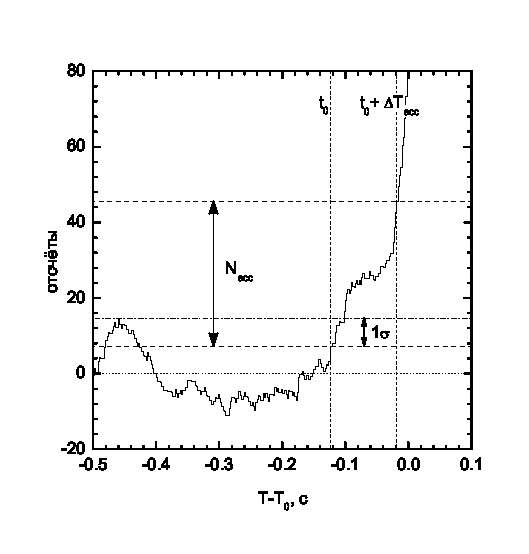
\includegraphics[width=1.0\textwidth]{gDurStartRU.eps} \\ а)}
  \end{minipage}
  \hfill
  \begin{minipage}[h]{0.5\textwidth}
    \center{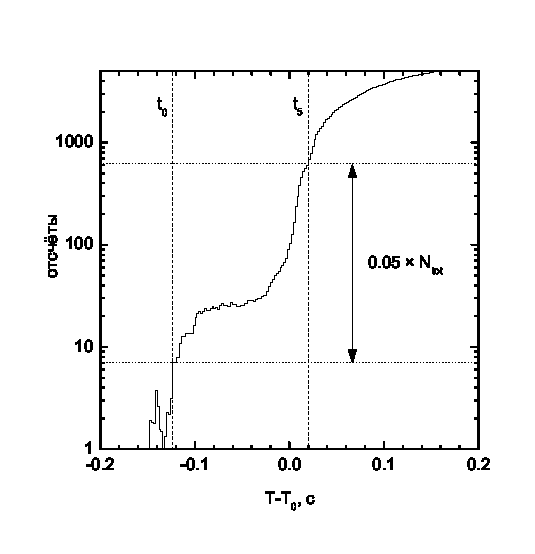
\includegraphics[width=1.0\textwidth]{gDurT5RU.eps} \\ б)}
  \end{minipage}  
  \caption{
  (а) Иллюстрация определения времени начала всплеска $t_0$ для GRB20031214\_T36655. 
  Сплошная линия~--- интегральное число отсчетов всплеска с вычетом фона. 
  Число отсчётов $N_\rmn{acc}$ (горизонтальные штриховые линии), 
  накопленное на интервале $\Delta T_\rmn{acc}$ (вертикальные штриховые линии), 
  соответствует превышению $5\sigma$ над фоном. Уровень $1\sigma$ относительно интегрального 
  числа отсчётов на момент $t_0$  изображен горизонтальной штрихпунктирной линией. 
  Горизонтальная точечная линия обозначает нулевой уровень.
  (б) Иллюстрация определения начала интервала $T_{90}$ ($t_5$) для того же всплеска.
  Число отсчётов, соответствующие 5\% от общего числа отсчётов $N_\rmn{tot}$ 
  обозначено горизонтальными штриховыми линиями, время начала всплеска $t_0$ и время $t_5$ 
  обозначены вертикальными штриховыми линиями. \label{fig:T100_calculation} }
\end{figure}

\subsection{Распределения по длительностям}
Для 1834 всплесков KW были построены гистограммы распределений всплесков по $T_{90}$ и $T_{50}$ 
для порогов значимости поиска начала и конца всплеска $4\sigma$, $5\sigma$ и $6\sigma$. 

Распределения  аппроксимировались методом минимизации $\chi^2$ суммой двух логнормальных распределений
\begin{equation}
f(x) = \sum_{l=1}^{2} A_l f_l(x) \mbox{ ,}
\end{equation}
где
\begin{equation}
f_l(x) = \frac{1}{w_l \sqrt{\pi/2}} \exp\left(\frac{-2(x-x_{cl})^2}{w_l^2}\right) \mbox{ ,}
\end{equation}
с параметрами $A_l$~--- площадь под распределением, $w=2\sigma$~--- ширина, $x_{cl}$~--- среднее значение и 
$x=\log T$. При этом число всплесков в бине по модели равно  интегралу от аппроксимирующей функции в границах бина. 

Доверительные интервалы параметров распределения на уровне 68\% вычислялись 
методом Mонте-Карло для 1000 реализаций распределения. При этом значение в каждом 
бине распределения разыгрывалось как пуассоновская случайной величиной со средним, равным 
числу отсчётов в соответствующем бине исходного распределения. Полученный набор 
значений каждого параметра распределения сортировался по возрастанию. В качестве нижней и верхней 
границы доверительного интервала на уровне 68\% из этого отсортированного массива 
параметров брались значения с индексами 160 и 840, соответственно. 
В качестве значения параметра бралась медиана распределения.

Из-за эффектов селекции число очень коротких всплесков ($T_{90} \lesssim 100$~мс) и 
число длинных всплесков ($T_{90} \gtrsim 200$~с) в наборе KW недооценено. Так же неверно 
считать ошибки числа отсчётов в бине гауссовыми при числе отсчётов $<10$, поэтому 
бины с $\log T_{90} \leq -1.2$ ($T_{90} \leq 0.063$~с) и $\log T_{90} \geq 2.4$ ($T_{90} \geq 251$~с) 
не учитывались при аппроксимации гистограммы распределения по $T_{90}$,  для аппроксимации 
использовалось 18 бинов. При аппроксимации гистограммы распределения по $T_{50}$ игнорировались 
бины c $\log T_{50} \leq -1.8$ ($T_{50} \leq 0.016$~с) и  $\log T_{50} \geq 2.0$ 
($T_{50} \geq 100$~с), для аппроксимации использовалось 19 бинов.

Параметры распределений представлены в таблицах~\ref{tab:T90_distr} и~\ref{tab:T50_distr}. 
Из представленных результатов видно, что при изменении порога от $4\sigma$ до $6\sigma$ 
параметры распределения по $T_{50}$ и $T_{90}$ для полного набора 1834 всплесков изменяются. 
Распределение длинных всплесков смещается в сторону меньших длительностей, такое же смещение, 
но в меньшей степени, наблюдается для распределение коротких всплесков. 
При этом изменение параметров распределения по $T_{90}$ гораздо существенней, 
чем для распределения по $T_{50}$, см. таб.~\ref{tab:Txx_vs_thd},
где $T_{\rmn{int}}$ соответствует пересечению распределений и 
$\delta T =|T_{4\sigma}-T_{6\sigma}| / T_{4\sigma}$. 
Так как вариации параметров распределения по $T_{50}$ существенно меньше, 
чем для распределения по $T_{90}$ для классификации всплесков на основе длительностей 
мы выбрали величину~$T_{50}$. 

\begin{table} [h]
 \centering
 \caption{Изменение параметров распределений $T_{90}$ и $T_{50}$ при изменении порога поиска от $4\sigma$ до $6\sigma$}
 \label{tab:Txx_vs_thd}
\scriptsize
%\rotate
  \begin{center}
  \begin{tabular}{c c c c c}
  \hline
  \hline
набор & величина & $\delta T_\rmn{c1}$ & $\delta T_\rmn{c2}$ & $\delta T_\rmn{int}$ \\
      &          &         (\%)        &   (\%)              &  (\%)            \\       
    
\hline
1834  &  $T_{90}$ &  19  & 27 &  14 \\ 
      &  $T_{50}$ &  7   & 13 &  4  \\ 
1168  &  $T_{90}$ &  26  & 21 &  15 \\ 
      &  $T_{50}$ &  7   & 10 &  6  \\
\hline
\end{tabular}
\end{center}
\end{table}

Вследствие наблюдательной селекции триггерной системы по отношению сигнал-шум 
наш набор всплесков неоднороден. Как видно из диаграммы $T_{50}$--$\rmn{S/N}$~(рис.~\ref{img:SNvsT50}) 
в наборе отсутствуют всплески с отношением сигнал-шум $\rmn{S/N} < 10$ и $T_{50} \lesssim 100$~мс. 
Здесь S/N определено как отношение числа отсчётов от источника к стандартному отклонению 
числа отсчётов фона на интервале 64~мс с максимальной скоростью счёта. 
Для дальнейшего рассмотрения был выбран однородный набор всплесков с $\rmn{S/N}\geq 10$, 
который содержит 1168 всплесков. 
Результаты аппроксимации распределений набора по $T_{50}$ и $T_{90}$ приведены в 
таблицах \ref{tab:T90_distr} и~\ref{tab:T50_distr}, и на рис.~\ref{img:T90andT50s5}. 
Относительные изменения параметров скорректированных распределений при изменении 
порога от $4\sigma$ до $6\sigma$ приведены в таб.~\ref{tab:Txx_vs_thd}. 

В качестве порога значимости был выбран уровень $5\sigma$ так как было замечено, 
что при пороге $4\sigma$ в качестве начала и конца всплеска часто выбираются 
флуктуации фона или эпизоды излучения транзиентов, не относящиеся ко всплеску  
(установить отношение подобных слабых эпизодов к триггерному всплеску в 
большинстве случаев не представляется возможным). При пороге $6\sigma$ часто 
игнорируется <<хвост>>, непосредственно прилегающий к основному пику, тем самым полное 
число отсчетов во всплеске может недооцениваться на величину до $\sim 70$\%.
Такая ситуация возможна, к примеру, для коротких всплесков с продлённым излучением.

В качестве границы между длинными и короткими всплесками была выбрана точка пересечения 
двух логнормальных распределений по $T_{50}$ для порога значимости $5\sigma$ 
набора 1168 всплесков $T_{50\rmn{,int}} = 0.6$~с. 

Для указанного распределения и границы между длинными и короткими всплесками 
можно оценить долю <<засорения>>\ набора коротких всплесков длинными и наоборот. 
Доля <<засорения>>\ набора коротких всплесков длинными равна отношению интеграла 
от распределения длинных всплесков и интеграла от распределения коротких всплесков 
на интервале $-\infty$ до $T_{50\rmn{int}}$) и составляет $\approx 7$\%. 
При этом доля <<засорения>>\ длинных всплесков короткими составляет~$\approx 2$\%.          

Границы диапазонов KW менялись со временем, что могло внести систематический 
сдвиг в длительности всплесков, зарегистрированных в различные периоды, и 
привести к изменению со временем границы между длинными и короткими всплесками. 
Для анализа дрейфа границы между длинными и короткими всплесками набор 1168 
всплесков был разделён на три поднабора: 583 GRBs ноябрь 1994~-- май 2003; 
585 GRBs июнь 2003~-- декабрь 2010; 582 GRBs  май 1999~-- январь 2007. 
Полученные для поднаборов границы $T_{50\rmn{int}}$ равны: 
$0.41_{-0.09}^{+0.19}$~c, 
$0.74_{-0.16}^{+0.22}$~c и 
$0.62_{-0.17}^{+0.28}$~c, соответственно. 
Наблюдаемый дрейф границы лежит в пределах $1\sigma$ интервала для границы $T_{50\rmn{int}} = 0.6$~с, 
полученной с использованием полного набора всплесков.

\begin{figure} [h] 
  \center
  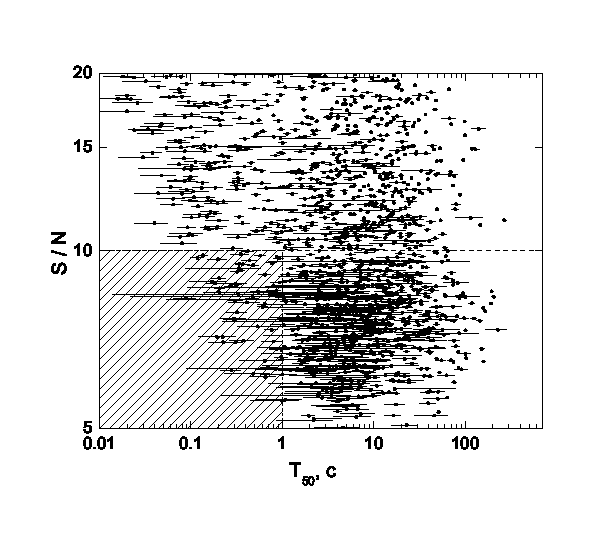
\includegraphics [width=0.75\textwidth] {gSNvsT50_ru}
  \caption[Соотношение S/N--$T_{50}$]{Соотношение S/N--$T_{50}$ для 1834 всплесков. 
  Пунктирная линия соответствует $\rmn{S/N}=10$. Штрихованная область наиболее подвержена 
  селекции триггерного алгоритма. Отношение сигнал-шум $\rmn{S/N}\geq 10$ имеют 1168 всплесков.} 
  \label{img:SNvsT50}  
\end{figure}

\begin{figure}[h]
  \begin{minipage}[h]{0.5\textwidth}
    \center{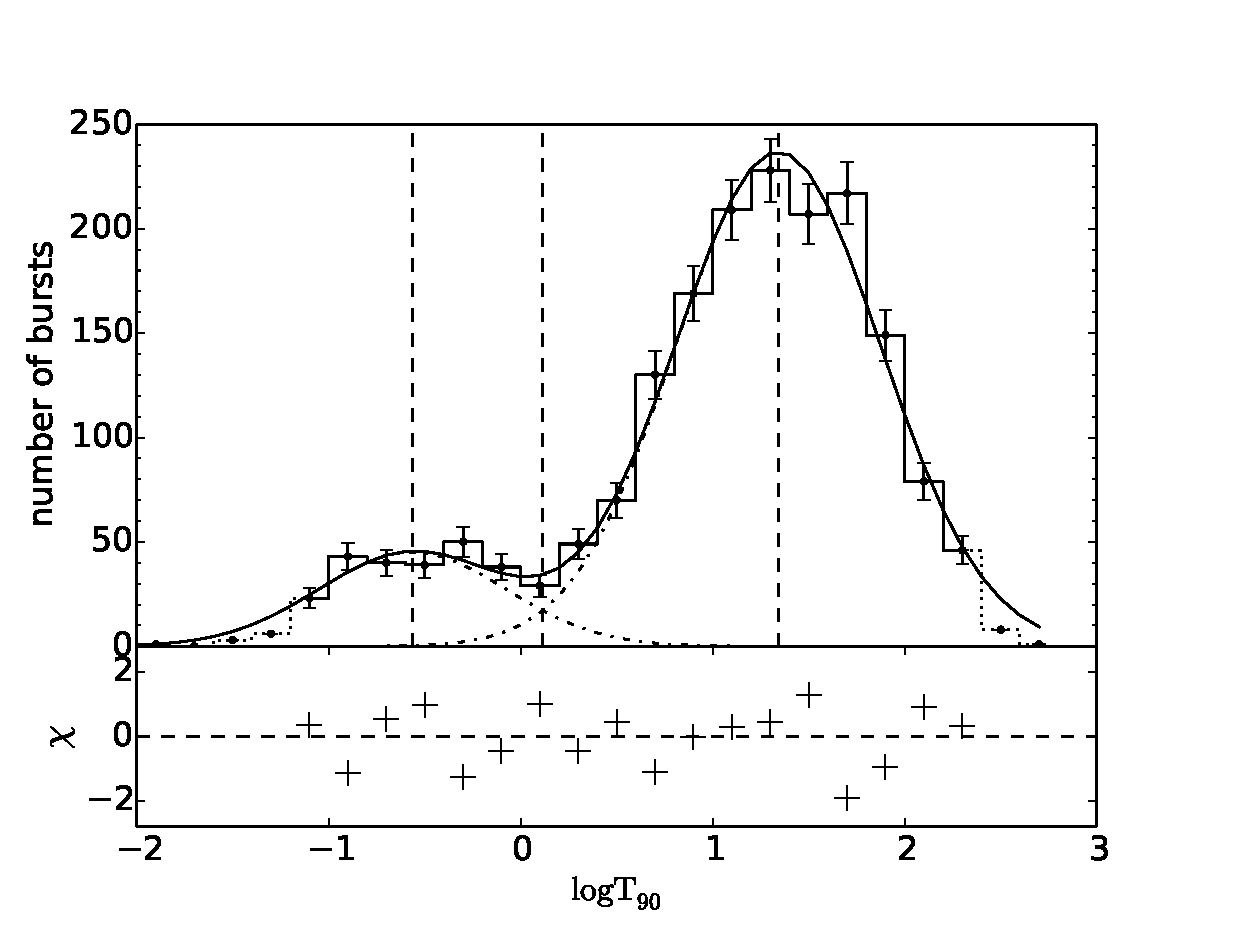
\includegraphics[width=1.0\textwidth]{dT90s5simple} \\ а)}
  \end{minipage}
  \hfill
  \begin{minipage}[h]{0.5\textwidth}
    \center{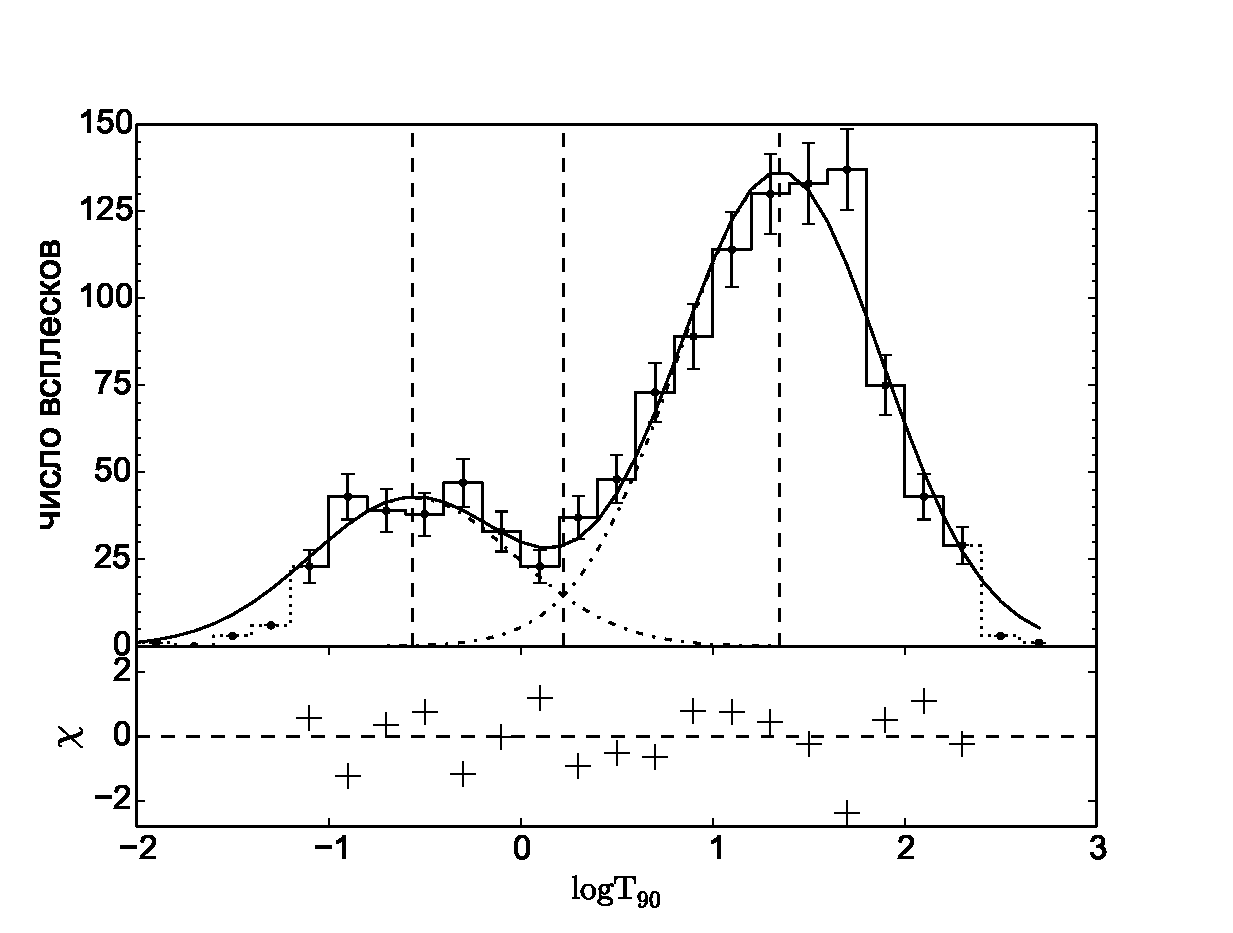
\includegraphics[width=1.0\textwidth]{dT90s5simple_SN10} \\ б)}
  \end{minipage}
  \vfill
  \begin{minipage}[h]{0.5\textwidth}
    \center{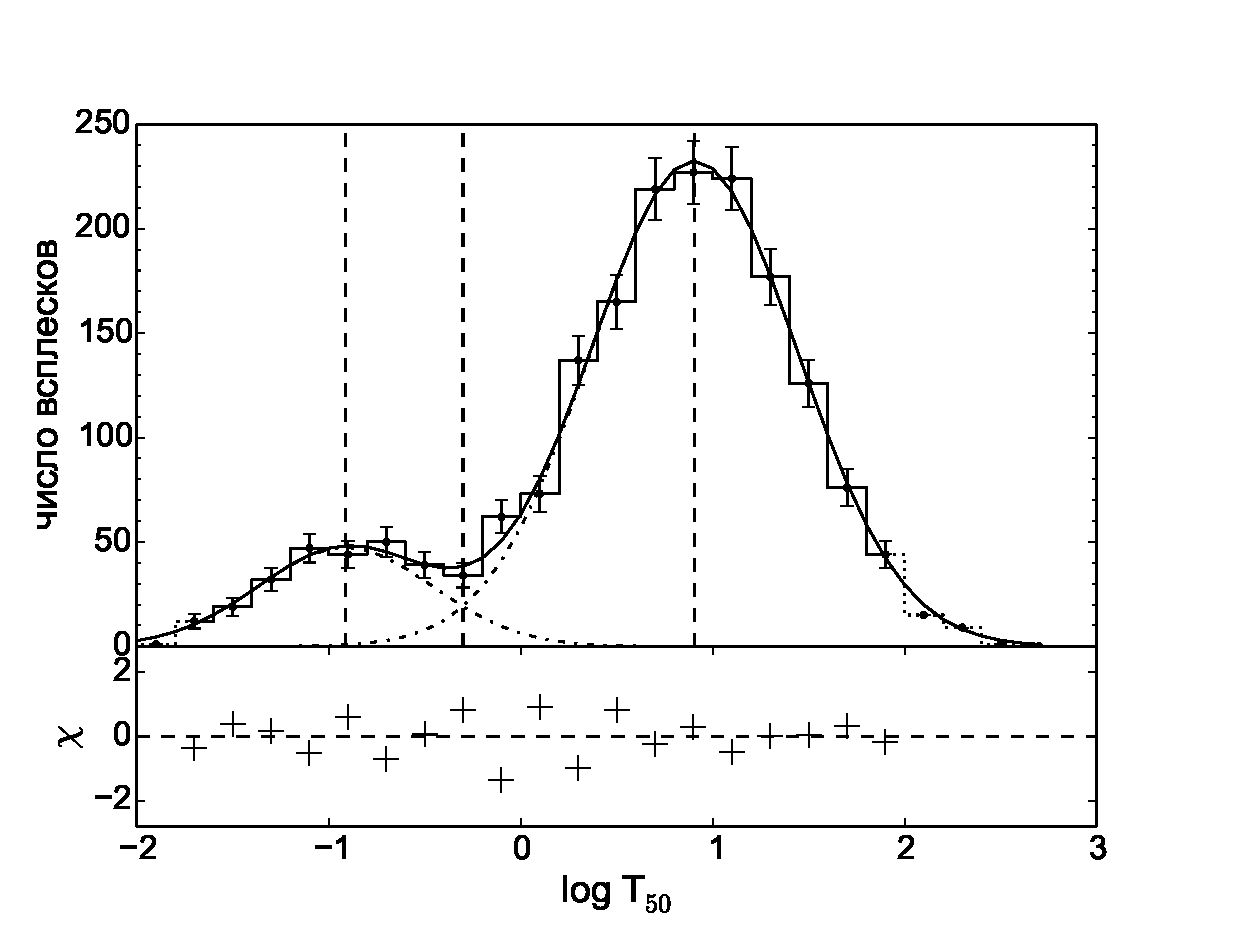
\includegraphics[width=1.0\textwidth]{dT50s5simple} \\ в)}
  \end{minipage}
  \hfill
  \begin{minipage}[h]{0.5\textwidth}
    \center{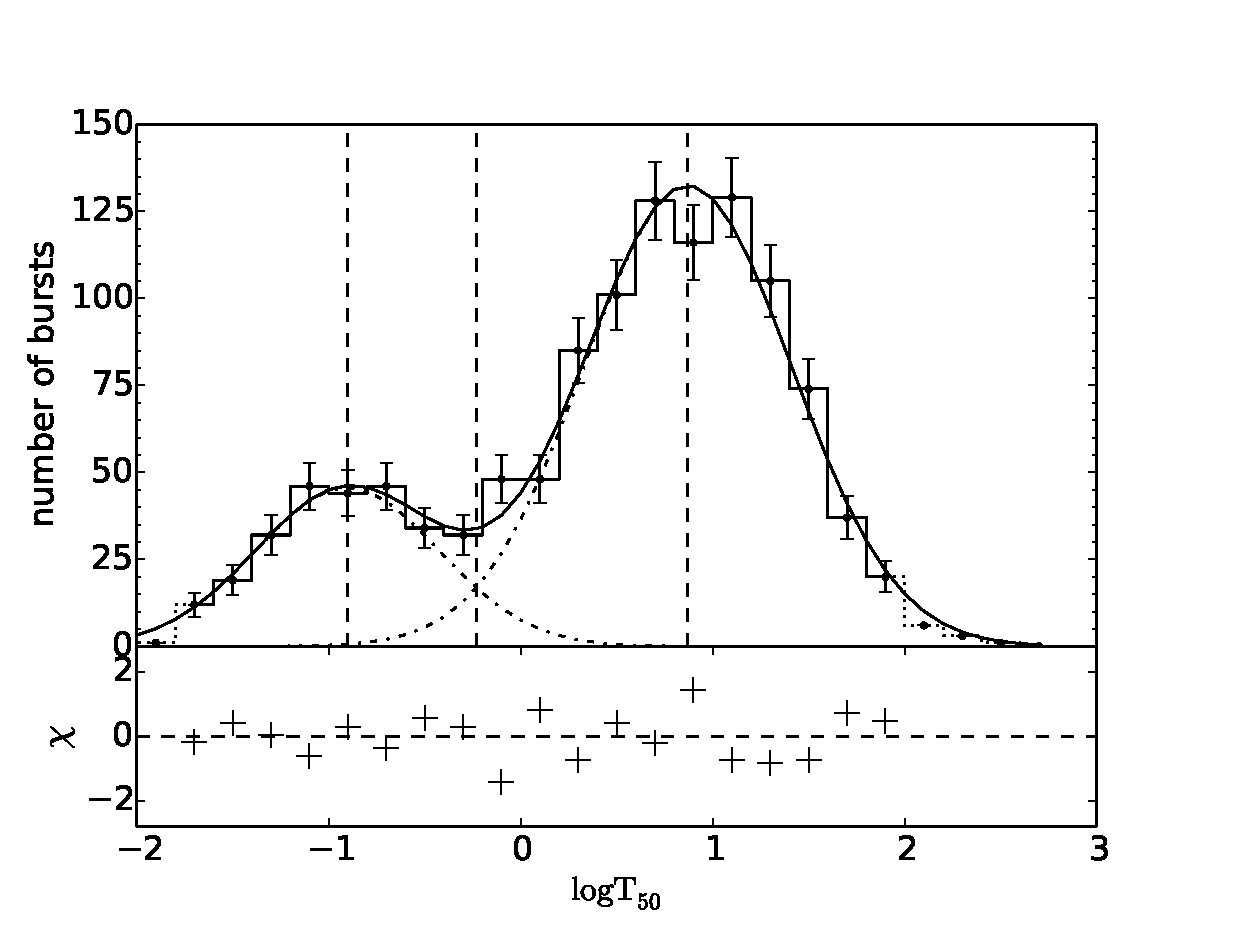
\includegraphics[width=1.0\textwidth]{dT50s5simple_SN10} \\ г)}
  \end{minipage}
  \caption[Распределения 1834 и 1168 всплесков с $\rmn{S/N}\geq 10$ по $T_{90}$ и~$T_{50}$]
  {Распределения 1834 и 1168 всплесков с $\rmn{S/N}\geq 10$ по $T_{90}$~(а и б, соответственно) и 
  $T_{50}$ (в и г, соответственно) для порога $5\sigma$ (непрерывная гистограмма), 
  игнорированные при аппроксимации бины гисторграммы показаны пунктиром. 
  Аппроксимация распределения суммой двух логнормальных распределений  показана 
  непрерывной линией, распределение коротких и длинных всплесков показаны 
  штрихпунктирными линиями.  Вертикальные штриховые лини обозначают средние значения 
  распределений коротких и длинных всплесков и точку их пересечения. 
  На нижней панели каждого рисунка показаны невязки аппроксимации.}
  \label{img:T90andT50s5}  
\end{figure}

\begin{landscape}
%\documentclass[preprint]{aastex}
%\usepackage{graphicx,natbib} 

%\begin{document}

\begin{table} [h]
 \centering
 \caption{Параметры аппроксимации распределений по $T_{90}$ для порогов 
          $4\sigma$, $5\sigma$ и $6\sigma$}\label{tab:T90_distr}
\scriptsize
%\rotate
  \begin{center}
  \begin{tabular}{c c c c c c c c c c c c c c} %14 col
  \hline
  \hline
число & $\sigma$ & $A_1$ & $xc_1$ & $T_{90c1}$ & $w_1$ & 
                 $A_2$ & $xc_2$ & $T_{90c2}$ & $w_2$ & 
				 $x_{\rmn{int}}$ & $T_{90\rmn{int}}$ & $\chi^2$ & dof \\
всплесков & & & & с & & & & с & & &  с & & \\
  \hline
%N_short = 243 N_long = 1591 N_tot = 1834
1834 & 4 & $     50 ^{+     6}_{-     5}$ & $  -0.49 ^{+  0.06}_{-  0.05}$ & $   0.32 ^{+  0.05}_{-  0.03}$ & $   0.92 ^{+  0.16}_{-  0.12}$ & $    324 ^{+     9}_{-    11}$ & $   1.44 ^{+  0.02}_{-  0.02}$ & $  27.30 ^{+  1.15}_{-  1.17}$ & $   1.11 ^{+  0.04}_{-  0.04}$ & $   0.15 ^{+  0.07}_{-  0.06}$ & $  1.42 ^{+ 0.26}_{- 0.19}$ &   10.5 & 12 \\ 
%N_short = 259 N_long = 1575 N_tot = 1834
& 5 & $     54 ^{+     8}_{-     6}$ & $  -0.56 ^{+  0.06}_{-  0.05}$ & $   0.27 ^{+  0.04}_{-  0.03}$ & $   0.97 ^{+  0.21}_{-  0.12}$ & $    316 ^{+     9}_{-    10}$ & $   1.34 ^{+  0.02}_{-  0.02}$ & $  22.09 ^{+  0.89}_{-  0.90}$ & $   1.06 ^{+  0.04}_{-  0.04}$ & $   0.11 ^{+  0.07}_{-  0.06}$ & $  1.30 ^{+ 0.24}_{- 0.16}$ &   14.6 & 12 \\ 
%N_short = 274 N_long = 1560 N_tot = 1834
& 6 & $     59 ^{+     8}_{-     6}$ & $  -0.59 ^{+  0.05}_{-  0.05}$ & $   0.26 ^{+  0.03}_{-  0.03}$ & $   0.95 ^{+  0.16}_{-  0.13}$ & $    312 ^{+     9}_{-    10}$ & $   1.30 ^{+  0.02}_{-  0.02}$ & $  20.00 ^{+  0.91}_{-  0.74}$ & $   1.07 ^{+  0.04}_{-  0.04}$ & $   0.09 ^{+  0.07}_{-  0.06}$ & $  1.22 ^{+ 0.22}_{- 0.15}$ &   10.3 & 12 \\ 
%N_short = 248 N_long = 920 N_tot = 1168
1168& 4 & $     53 ^{+    11}_{-     7}$ & $  -0.47 ^{+  0.10}_{-  0.06}$ & $   0.34 ^{+  0.09}_{-  0.05}$ & $   1.03 ^{+  0.31}_{-  0.18}$ & $    182 ^{+    10}_{-    12}$ & $   1.42 ^{+  0.03}_{-  0.03}$ & $  26.41 ^{+  2.12}_{-  1.85}$ & $   1.07 ^{+  0.07}_{-  0.08}$ & $   0.28 ^{+  0.15}_{-  0.12}$ & $  1.91 ^{+ 0.81}_{- 0.45}$ &   13.2 & 12 \\ 
%N_short = 264 N_long = 904 N_tot = 1168
S/N$>$10 & 5 & $     58 ^{+    10}_{-     8}$ & $  -0.57 ^{+  0.08}_{-  0.07}$ & $   0.27 ^{+  0.05}_{-  0.04}$ & $   1.09 ^{+  0.29}_{-  0.20}$ & $    178 ^{+     9}_{-    10}$ & $   1.35 ^{+  0.03}_{-  0.03}$ & $  22.51 ^{+  1.74}_{-  1.41}$ & $   1.05 ^{+  0.06}_{-  0.06}$ & $   0.23 ^{+  0.13}_{-  0.10}$ & $  1.71 ^{+ 0.58}_{- 0.36}$ &   15.5 & 12 \\ 
%N_short = 278 N_long = 890 N_tot = 1168
& 6 & $     61 ^{+    12}_{-     7}$ & $  -0.60 ^{+  0.06}_{-  0.06}$ & $   0.25 ^{+  0.04}_{-  0.04}$ & $   1.04 ^{+  0.29}_{-  0.16}$ & $    175 ^{+     7}_{-    10}$ & $   1.32 ^{+  0.03}_{-  0.03}$ & $  20.79 ^{+  1.54}_{-  1.28}$ & $   1.04 ^{+  0.06}_{-  0.06}$ & $   0.21 ^{+  0.11}_{-  0.10}$ & $  1.63 ^{+ 0.49}_{- 0.32}$ &   16.1 & 12 \\ 
\hline
\end{tabular}
\end{center}
\end{table}

\begin{table} [h]
 \centering
 \caption{Параметры аппроксимации распределений по $T_{50}$ для порогов 
          $4\sigma$, $5\sigma$ и $6\sigma$}\label{tab:T50_distr}
\scriptsize
%\rotate
  \begin{center}
  \begin{tabular}{c c c c c c c c c c c c c c}
  \hline
  \hline
число & $\sigma$ & $A_1$ & $xc_1$ & $T_{50c1}$ & $w_1$ & 
                             $A_2$ & $xc_2$ & $T_{50c2}$ & $w_2$ & 
							 $x_{\rmn{int}}$ & $T_{50\rmn{int}}$ & $\chi^2$ & dof \\
							 
всплесков & & & & с & & & & с & & &  с & & \\
\hline
%N_short = 252 N_long = 1582 N_tot = 1834
1834 & 4 & $     50 ^{+     5}_{-     4}$ & $  -0.86 ^{+  0.05}_{-  0.05}$ & $   0.14 ^{+  0.02}_{-  0.01}$ & $   0.86 ^{+  0.10}_{-  0.09}$ & $    312 ^{+     9}_{-     9}$ & $   0.95 ^{+  0.02}_{-  0.02}$ & $   8.86 ^{+  0.36}_{-  0.35}$ & $   1.06 ^{+  0.04}_{-  0.04}$ & $  -0.26 ^{+  0.06}_{-  0.06}$ & $  0.54 ^{+ 0.08}_{- 0.07}$ &   14.7 & 13 \\ 
%N_short = 263 N_long = 1571 N_tot = 1834
& 5 & $     53 ^{+     6}_{-     5}$ & $  -0.91 ^{+  0.05}_{-  0.05}$ & $   0.12 ^{+  0.02}_{-  0.01}$ & $   0.89 ^{+  0.12}_{-  0.10}$ & $    311 ^{+    10}_{-     9}$ & $   0.91 ^{+  0.02}_{-  0.02}$ & $   8.06 ^{+  0.35}_{-  0.33}$ & $   1.07 ^{+  0.04}_{-  0.04}$ & $  -0.30 ^{+  0.07}_{-  0.06}$ & $  0.50 ^{+ 0.09}_{- 0.07}$ &    6.9 & 13 \\ 
%N_short = 278 N_long = 1556 N_tot = 1834
& 6 & $     57 ^{+     6}_{-     5}$ & $  -0.89 ^{+  0.06}_{-  0.05}$ & $   0.13 ^{+  0.02}_{-  0.02}$ & $   0.93 ^{+  0.12}_{-  0.10}$ & $    307 ^{+    10}_{-     9}$ & $   0.89 ^{+  0.02}_{-  0.02}$ & $   7.73 ^{+  0.35}_{-  0.34}$ & $   1.07 ^{+  0.04}_{-  0.04}$ & $  -0.28 ^{+  0.07}_{-  0.07}$ & $  0.52 ^{+ 0.09}_{- 0.08}$ &    8.4 & 13 \\ 
%N_short = 256 N_long = 912 N_tot = 1168
1168 &4 & $     51 ^{+     6}_{-     5}$ & $  -0.85 ^{+  0.07}_{-  0.06}$ & $   0.14 ^{+  0.02}_{-  0.02}$ & $   0.92 ^{+  0.13}_{-  0.12}$ & $    178 ^{+     8}_{-     9}$ & $   0.91 ^{+  0.03}_{-  0.03}$ & $   8.07 ^{+  0.55}_{-  0.51}$ & $   1.05 ^{+  0.06}_{-  0.05}$ & $  -0.19 ^{+  0.09}_{-  0.09}$ & $  0.65 ^{+ 0.15}_{- 0.12}$ &   15.8 & 13 \\ 
%N_short = 263 N_long = 905 N_tot = 1168
S/N$>$10 &  5 & $     54 ^{+     7}_{-     6}$ & $  -0.90 ^{+  0.08}_{-  0.06}$ & $   0.12 ^{+  0.03}_{-  0.01}$ & $   0.94 ^{+  0.17}_{-  0.12}$ & $    178 ^{+     7}_{-     9}$ & $   0.87 ^{+  0.03}_{-  0.03}$ & $   7.43 ^{+  0.58}_{-  0.51}$ & $   1.07 ^{+  0.06}_{-  0.06}$ & $  -0.23 ^{+  0.11}_{-  0.09}$ & $  0.59 ^{+ 0.17}_{- 0.11}$ &    9.3 & 13 \\ 
%N_short = 278 N_long = 890 N_tot = 1168
& 6 & $     56 ^{+     7}_{-     6}$ & $  -0.89 ^{+  0.07}_{-  0.06}$ & $   0.13 ^{+  0.02}_{-  0.02}$ & $   0.96 ^{+  0.14}_{-  0.11}$ & $    175 ^{+     7}_{-     8}$ & $   0.86 ^{+  0.03}_{-  0.03}$ & $   7.29 ^{+  0.52}_{-  0.48}$ & $   1.06 ^{+  0.06}_{-  0.05}$ & $  -0.21 ^{+  0.09}_{-  0.08}$ & $  0.61 ^{+ 0.15}_{- 0.11}$ &    9.6 & 13 \\ 
\hline
\end{tabular}
\end{center}
\end{table}
%\end{document}

\end{landscape}

\subsection{Сравнение длительностей определенных по данным BATSE и KW}
Среди 1939 всплесков KW без сбоев 267 всплесков наблюдались BATSE. 
Соотношение длительностей $T_{50}$ и $T_{90}$, вычисленных по данным BATSE~\citep{Paciesas_1999} 
и KW, изображено на рис.~\ref{img:T90andT50_KWvsBATSE}.

Большинство всплесков имеют б\'{о}льшую длительность по данным BATSE, 
в особенности $T_{90}$ по сравнению с KW, что связано с большей  эффективной площадью детекторов 
BATSE $\sim 10^3$~см$^2$ против $(0.80\textrm{--}1.6)\times 10^2$~см$^2$ у KW. 
Другим фактором является то, что длительность всплесков BATSE определяется в 
диапазоне $>25$~кэВ, что позволяет учитывать продолжительные мягкие хвосты всплесков. 
Более редкой ситуацией является существенное превышение длительностей по данным KW, 
наблюдаемое в 10 всплесках. Шесть всплесков имеют плавное спадание/нарастание интенсивности, 
которое не было учтено при вычислении  длительностей по данным BATSE, возможно, 
из-за недостаточно точной аппроксимации фона. В трех всплесках по данным KW
в интервал $T_{90}$ попадает слабый импульс, отделенный от основного пика. 
При этом эклиптические широты основного пика и слабого импульса согласуются, 
что позволяет отнести их к одному источнику. Во всплеске GRB~950904, 
$T_{0\rmn{,BATSE}} = 52777$~s~UT ($T_{90\rmn{,KW}} = 99 \pm 4$~с, $T_{90\rmn{,BATSE}} = 11.1\pm 1.8$~с) 
длительности BATSE даны для второго импульса, так как в~\citep{Hurley_2005} полагается, 
что два импульса являются различными всплесками.

Среди общих всплесков KW и BATSE 46 имеют $T_{50\rmn{KW}} \leq 0.6$~с, 
из них 9 входят в набор 105 всплесков с искаженной длительностью (см.~Раздел~\ref{sec:GRB_sample}). 
Из оставшихся 37, 8 имеют $T_{90\rmn{BATSE}} > 2$~с, 
из них один является короткими всплеском с продлённым излучением. Таким образом, 
засорение нашего списка длинными всплесками, связанное с низким S/N всплесков KW
по сравнению с BATSE, составляет 19\% (=7/37). % без учета всплесков с продлённым излучением. 
Ранее в работе~\citep{Ofek_2007ApJ} была получена доля 
<<засорения>> коротких всплесков KW длинными $\approx 60$\%. В этой работе
длительность всплесков в данных KW оценивалась визуально, что могло 
стать причиной получения высокой доли засорения. 

\begin{figure}[h]
  \begin{minipage}[h]{0.5\textwidth}
    \center{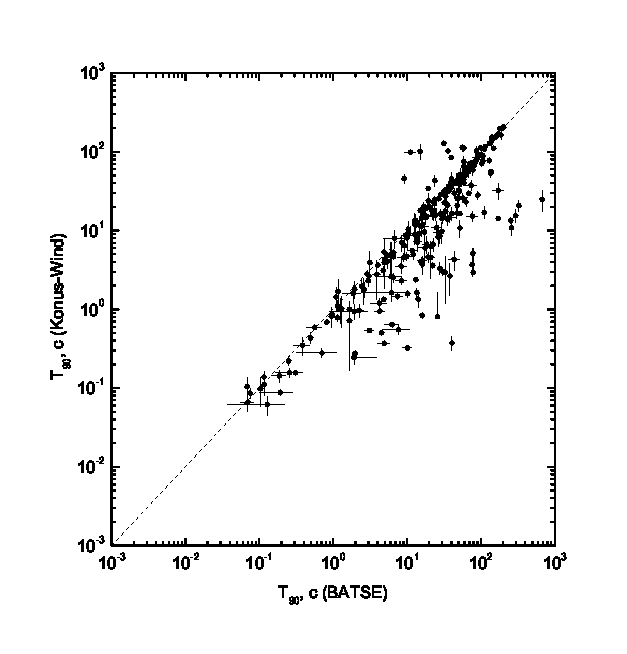
\includegraphics[width=1.0\textwidth]{gT90_KWvsBATSE_ru} \\ а)}
  \end{minipage}
  \hfill
  \begin{minipage}[h]{0.5\textwidth}
    \center{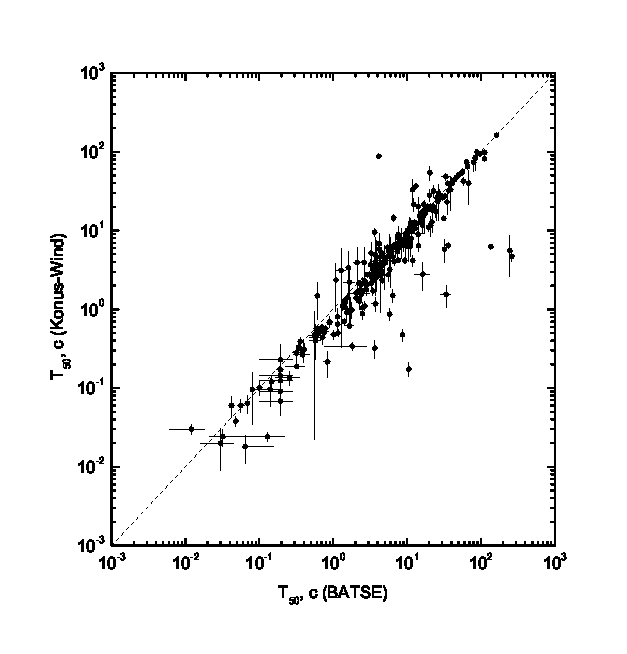
\includegraphics[width=1.0\textwidth]{gT50_KWvsBATSE_ru} \\ б)}
  \end{minipage}
  \caption{Соотношение длительностей $T_{90}$~(a) и $T_{50}$~(б), определённых по 
  данным BATSE и KW для 267 гамма-всплесков.}
  \label{img:T90andT50_KWvsBATSE}  
\end{figure}

\subsection{Набор коротких всплесков}
Набор из 1834 всплесков KW содержит 277 событий с $T_{50} \leq 0.6$~с.    %<-- число 277 проверено
Среди них было обнаружено: пять очевидно длинных всплесков, в которых $T_{50}$ 
% (ID = 1122, 2196, 2922, 2184) и ID=1228 $T_{90} = 8$~с в данных SAX
определялось наиболее сильным импульсом, при этом полная длительность всплеска была 
значительно больше 2~с; и 12 кандидатов в короткие всплески с продлённым излучением.
Визуальный анализ показал, что среди 69 всплесков со сбоями пять имеют $T_{50} \leq 0.6$~с, 
эти всплески были включены в итоговый набор. 
% ID = 243, 704, 882 (солн. вспышка в данных), 934, 3319 (пропущен ранее)
Таким образом, набор коротких всплесков KW содержит 265 событий без продлённого излучения.

Кроме того, было обнаружено 19 кандидатов во всплески с продлённым излучением среди всплесков с $T_{50} > 0.6$~с. 
К этому типу всплесков были отнесены события, имеющие короткий начальный импульс с $T_{50} \leq 0.6$~с, 
за которым следует эпизод излучения, не содержащий импульсов с заметной спектральной эволюцией. 
В некоторых случаях начальный пик и продлённое излучение были разделены интервалом, 
на котором интенсивность излучения мала. Таким образом, полученный набор коротких всплесков с 
продлённым излучением насчитывает 31 событие.

Объединённый набор коротких всплесков с учётом всплесков с продлённым излучением 
содержит 296 событий.
\FloatBarrier

\section{Жесткости}\label{sec:Hardness}
Для анализа спектральных различий всплесков использовалось две величины: интегральная 
жёсткость ($\rmn{HR}_{32}$)~--- отношение числа отсчетов, накопленных в каналах G3 и G2 
за интервал $T_{100}$ и пиковая жёсткость ($\rmn{HR}_{32\rmn{pk}}$)~--- отношение числа отсчетов, 
накопленных за интервал 64~мс с пиковой скоростью счета. 
Отношение числа отсчётов в каналах G3 и G2 было выбрано, так как 
оно наименее чувствительно к углу падения на детектор и более чувствительно 
к пиковой энергии $E_\rmn{p}$.  

При вычислении жесткости $\rmn{HR}_{32}$ был учтён временн\'{о}й дрейф границ диапазонов. 
Для этого трёхканальный спектр отсчётов аппроксимировался степенной функцией 
с экспоненциальным завалом $dN/dE \propto E^{\alpha} \exp(-E/E_0)$. 
С использованием полученной аппроксимации, вычислялось количество отсчётов в номинальных 
границах диапазонов: 13--50~кэВ~(G1), 50--200~кэВ~(G2) и 200--750~кэВ~(G3). 
Реальные границы диапазонов были вычислены с использованием калибровки, полученной 
по многоканальному спектру (см. Главу~\ref{KW_description}).

При рассмотрении интегральной жесткости использовался однородный набор из 1168 
всплесков с $\rmn{S/N} \geq 10$. Набор содержит восемь всплесков со сбоями в G1, 
для которых невозможно провести аппроксимацию трёхканального спектра. 
Из оставшихся всплесков, 17 имеют значительную ошибку $\rmn{HR}_{32}$ 
($\sigma\rmn{HR}_{32}/\rmn{HR}_{32} >0.3$), эти всплески были исключены из рассмотрения. 
В итоге для исследования соотношения жёсткость-длительность использовалось 1143 всплеска.

Распределение этого набора всплесков по $\rmn{HR}_{32}$ хорошо описывается суммой двух 
лог-нормальных распределений. Добавление третьей компоненты не даёт существенного 
улучшения аппроксимации. 

Аналогично работе~\citep{Horvath_2006} распределения всплесков на 
плоскости $\log T_{50}$--$\log \rmn{HR}_{32}$ аппроксимировалось суммой двух и трёх 
гауссовых компонент, при помощи метода наибольшего правдоподобия. Каждая компонента имеет вид: 
\begin{equation}
p(x,y| l) = \frac{1}{2\pi \sigma_x \sigma_y \sqrt{1-r^2}} \times 
\exp\left[ -\frac{1}{2(1-r^2)}\left( \frac{(x-a_x)^2}{\sigma_x^2} + 
\frac{(y-a_y)^2}{\sigma_y^2} -\frac{C}{\sigma_x \sigma_y}\right)\right]\mbox{ ,}
\end{equation}
где
\begin{equation}
C = 2r(x-a_x)(y-a_y)\mbox{ ,} \nonumber
\end{equation}
где $x=\log T_{50}$ и $y=\log \mbox{HR}_{32}$,  $a_x$, $a_y$~--- средние, 
$\sigma_x$, $\sigma_y$~--- дисперсии, $r$~--- коэффициент корреляции, 
и $l$~--- номер компоненты. При этом функция правдоподобия определяется следующим образом:
\begin{equation}
L = \sum_i \ln p(x_i, y_i)\mbox{ ,}
\end{equation}
где
\begin{equation}
p(x,y) = \sum_l  p(x, y|l)p_l \nonumber
\end{equation}
Аппроксимация производилась с помощью алгоритма 
expectation maximization~\citep{Horvath_2006, Balazs_2003AA} реализованного в пакете 
Scikit-learn~\citep{scikit-learn}. 
Ошибки параметров вычислялись таким же методом, как и для распределения по длительностям. 
На каждой из 1000 итераций генерировалось распределение на плоскости  
$\log T_{50}$--$\log\rmn{HR}_{32}$ на основе ошибок $T_{50}$ и $\rmn{HR}_{32}$. 
Затем из полученного массива параметров в качестве центрального значения и ширины доверительного 
интервала бралась медиана и ширина на уровне 68\%. Значения параметров гауссовых компонент 
для случая двух и трёх компонент представлены в таблицах~\ref{tab:clusters2_HR} 
и~\ref{tab:clusters3_HR}, расположение компонент представлено на рис.~\ref{img:HRvsT50}. 

Различие значений функций правдоподобия для двух компонент $L_2 = -1243$ и трёх 
компонент $L_3 = -1219$ ($\Delta L = 24$). Как показано в~\citep{Horvath_2006} 
в этом случае $2\Delta L$ распределено как $\chi^2_6$ и вероятность случайного 
отклонения $2\Delta L = 48$ равна $10^{-8}$. Функция правдоподобия для четырёх 
компонент $L_4 = -1211$, $2(L_4 - L_3) = 16$ вероятность получения этой величины случайным образом равна $0.01$. 
Это свидетельствует о наличии не более трёх классов всплесков. Третий класс всплесков 
значительно перекрывается с классом длинных/мягких всплесков (см. Рис.~\ref{img:HRvsT50}), поэтому нельзя утверждать, 
что он соответствует реальному физически выделенному классу всплесков, а не вызван эффектами селекции. 
Также, учитывая, что распределения по $T_{50}$ и $\rmn{HR}_{32}$ сами по себе описываются 
только двумя компонентами, для дальнейшего описания набора всплесков KW была выбрана
сумма только двух компонент, которые далее именуются короткие/жесткие и длинные/мягкие всплески.

Принадлежность всплеска к классу с номером $l$ определяется на основании значения индикаторной функции
\begin{equation}
I_l =\frac{p_l p(x,y|l)}{\sum_l  p(x, y|l)}
\end{equation}
Используя индикаторную функцию кластера коротких/жестких всплесков $I$, 
всплески были классифицированы следующим образом: 
$I \geq 0.9$~--- Тип~I, $0.1 \leq I < 0.9$~--- Тип~I/II (неопределённый тип), 
$I < 0.1$~--- Тип~II. Названия типов выбраны по аналогии с физической классификацией. 
Результаты классификации представлены на Рис~\ref{img:HRvsT50Types}.

В наборе 1143 всплесков доли всплесков разных типов составляют: Тип~I~--- 18\%,
Тип~I/II~--- 4\% и Тип~II~--- 78\%. Для всех всплесков типа~I длительность согласуется 
с ограничением $T_{50} \leq 0.6$~с. Доля всплесков типа~II среди коротких всплесков 
составляет 7\% (19\% если всплески типа~I/II относятся к типу~II), что согласуется с долей
<<засорения>> коротких всплесков длинными, вычисленной только на основе распределения 
по длительностям. Для временных историй коротких всплесков типа~II характерно 
наличие одного импульса с плавным нарастанием и спадом.
Из 31-го кандидата в короткие всплески с EE начальные импульсы 21-го события 
имеют Тип~I (далее Iee) и 10 имеют неопределённый тип (далее Iee/II).
При этом начальные импульсы двух событий, отнесённых к всплескам с EE, имеют тип~II.   % ID = 554, 2225

Также был произведён анализ распределения длительность-пиковая жёсткость. 
Для этого использовались 1104 GRBs с $\rmn{S/N} \geq 10$ и $\sigma \rmn{HR}_{32\rmn{pk}}/\rmn{HR}_{32\rmn{pk}} <0.3$. 
Результаты аппроксимации двумя и тремя гауссовыми компонентами приведены на рис.~\ref{img:HRpkvsT50}. 
Параметры распределений приведены в таблице~\ref{tab:tab_2clusters_HRpk} и~\ref{tab:tab_3clusters_HRpk}. 
Различие в жесткостях длинных и коротких всплесков составляет примерно 1.7 раза для пиковых 
жесткостей и 2.4 раза для интегральных. 

%\documentclass[preprint]{aastex}
%\usepackage{graphicx,natbib} 
%
%\begin{document}

\begin{table} [h]
 \centering
 \caption{Параметры распределения $\log T_{50}$--$\log \rmn{HR}_{32}$, в случае $k=2$}\label{tab:clusters2_HR}
\scriptsize

  \begin{center}
  \begin{tabular}{c c c c c c c c c}
  \hline
  \hline
$l$  &  $a_x$ &  $T_{50c}$ (c) &  $a_y$ &   $\rmn{HR}_c$ &  $\sigma_x$ &  $\sigma_y$ &  $r$ &  $p_l$\\
  \hline
1 & $-0.940_{-  0.012}^{+  0.032}$ & $   0.115_{-  0.003}^{+  0.009}$ & $-0.124_{-  0.019}^{+  0.011}$ & $   0.752_{-  0.032}^{+  0.020}$ & $ 0.442_{-  0.015}^{+  0.033}$ & $ 0.221_{-  0.010}^{+  0.008}$ & $ 0.020_{-  0.056}^{+  0.041}$ & $ 0.210_{-  0.003}^{+  0.011}$\\
2 & $ 0.835_{-  0.005}^{+  0.017}$ & $   6.834_{-  0.081}^{+  0.265}$ & $-0.499_{-  0.002}^{+  0.001}$ & $   0.317_{-  0.002}^{+  0.001}$ & $ 0.560_{-  0.019}^{+  0.003}$ & $ 0.216_{-  0.003}^{+  0.003}$ & $ 0.176_{-  0.008}^{+  0.006}$ & $ 0.791_{-  0.012}^{+  0.002}$\\
  \hline
\end{tabular}
\end{center}
\end{table}

\begin{table} [h]
 \centering
 \caption{Параметры распределения $\log T_{50}$--$\log \rmn{HR}_{32}$, в случае $k=3$}\label{tab:clusters3_HR}
\scriptsize

  \begin{center}
  \begin{tabular}{c c c c c c c c c}
  \hline
  \hline
$l$  &  $a_x$ &  $T_{50c}$ (c) &  $a_y$ &   $\rmn{HR}_c$ &  $\sigma_x$ &  $\sigma_y$ &  $r$ &  $p_l$\\
  \hline
1 & $-0.962_{-  0.016}^{+  0.008}$ & $   0.109_{-  0.004}^{+  0.002}$ & $-0.058_{-  0.013}^{+  0.003}$ & $   0.876_{-  0.026}^{+  0.005}$ & $ 0.414_{-  0.018}^{+  0.019}$ & $ 0.168_{-  0.016}^{+  0.007}$ & $ 0.098_{-  0.056}^{+  0.020}$ & $ 0.170_{-  0.010}^{+  0.009}$\\
2 & $ 0.088_{-  0.115}^{+  0.129}$ & $   1.224_{-  0.284}^{+  0.424}$ & $-0.583_{-  0.023}^{+  0.019}$ & $   0.261_{-  0.013}^{+  0.012}$ & $ 0.739_{-  0.030}^{+  0.031}$ & $ 0.264_{-  0.004}^{+  0.023}$ & $-0.176_{-  0.112}^{+  0.063}$ & $ 0.187_{-  0.017}^{+  0.006}$\\
3 & $ 0.949_{-  0.012}^{+  0.004}$ & $   8.886_{-  0.237}^{+  0.083}$ & $-0.468_{-  0.004}^{+  0.005}$ & $   0.340_{-  0.003}^{+  0.004}$ & $ 0.487_{-  0.003}^{+  0.005}$ & $ 0.194_{-  0.003}^{+  0.001}$ & $ 0.071_{-  0.004}^{+  0.009}$ & $ 0.654_{-  0.022}^{+  0.010}$\\
\hline
\end{tabular}
\end{center}
\end{table}

\begin{table} [h]
 \centering
 \caption{Параметры распределения $\log T_{50}$--$\log \rmn{HR}_{32\rmn{pk}}$, в случае $k=2$}\label{tab:tab_2clusters_HRpk}
\scriptsize

  \begin{center}
  \begin{tabular}{c c c c c c c c c}
  \hline
  \hline
  $l$  &  $a_x$ &  $T_{50c}$ (c) &  $a_y$ &   $\rmn{HR}_c$ &  $\sigma_x$ &  $\sigma_y$ &  $r$ &  $p_l$\\
  \hline
1 & $-0.948_{-  0.012}^{+  0.025}$ & $   0.113_{-  0.003}^{+  0.007}$ & $-0.068_{-  0.008}^{+  0.008}$ & $   0.856_{-  0.016}^{+  0.016}$ & $ 0.422_{-  0.015}^{+  0.009}$ & $ 0.260_{-  0.008}^{+  0.002}$ & $ 0.112_{-  0.045}^{+  0.020}$ & $ 0.214_{-  0.003}^{+  0.003}$\\
2 & $ 0.842_{-  0.006}^{+  0.004}$ & $   6.954_{-  0.097}^{+  0.059}$ & $-0.286_{-  0.001}^{+  0.006}$ & $   0.517_{-  0.001}^{+  0.007}$ & $ 0.550_{-  0.004}^{+  0.001}$ & $ 0.248_{-  0.001}^{+  0.007}$ & $ 0.191_{-  0.013}^{+  0.002}$ & $ 0.786_{-  0.003}^{+  0.003}$\\
\hline
\end{tabular}
\end{center}
\end{table}

\begin{table} [h]
 \centering
 \caption{Параметры распределения $\log T_{50}$--$\log \rmn{HR}_{32\rmn{pk}}$, в случае $k=3$}\label{tab:tab_3clusters_HRpk}
\scriptsize

  \begin{center}
  \begin{tabular}{c c c c c c c c c}
  \hline
  \hline
  $l$  &  $a_x$ &  $T_{50c}$ (c) &  $a_y$ &   $\rmn{HR}_c$ &  $\sigma_x$ &  $\sigma_y$ &  $r$ &  $p_l$\\
  \hline
1 & $-0.992_{-  0.021}^{+  0.023}$ & $   0.102_{-  0.005}^{+  0.005}$ & $-0.005_{-  0.026}^{+  0.025}$ & $   0.988_{-  0.058}^{+  0.059}$ & $ 0.411_{-  0.027}^{+  0.026}$ & $ 0.200_{-  0.016}^{+  0.021}$ & $ 0.213_{-  0.065}^{+  0.055}$ & $ 0.175_{-  0.022}^{+  0.019}$\\
2 & $ 0.298_{-  0.241}^{+  0.207}$ & $   1.988_{-  0.848}^{+  1.216}$ & $-0.394_{-  0.028}^{+  0.022}$ & $   0.404_{-  0.025}^{+  0.021}$ & $ 0.737_{-  0.094}^{+  0.082}$ & $ 0.291_{-  0.015}^{+  0.018}$ & $ 0.009_{-  0.175}^{+  0.136}$ & $ 0.251_{-  0.051}^{+  0.078}$\\
3 & $ 0.964_{-  0.030}^{+  0.038}$ & $   9.210_{-  0.607}^{+  0.834}$ & $-0.243_{-  0.010}^{+  0.013}$ & $   0.572_{-  0.013}^{+  0.017}$ & $ 0.476_{-  0.016}^{+  0.016}$ & $ 0.215_{-  0.013}^{+  0.007}$ & $ 0.104_{-  0.044}^{+  0.029}$ & $ 0.579_{-  0.102}^{+  0.063}$\\
\hline
\end{tabular}
\end{center}
\end{table}
%\end{document}

\begin{figure}[h]
  \begin{minipage}[h]{0.5\textwidth}
    \center{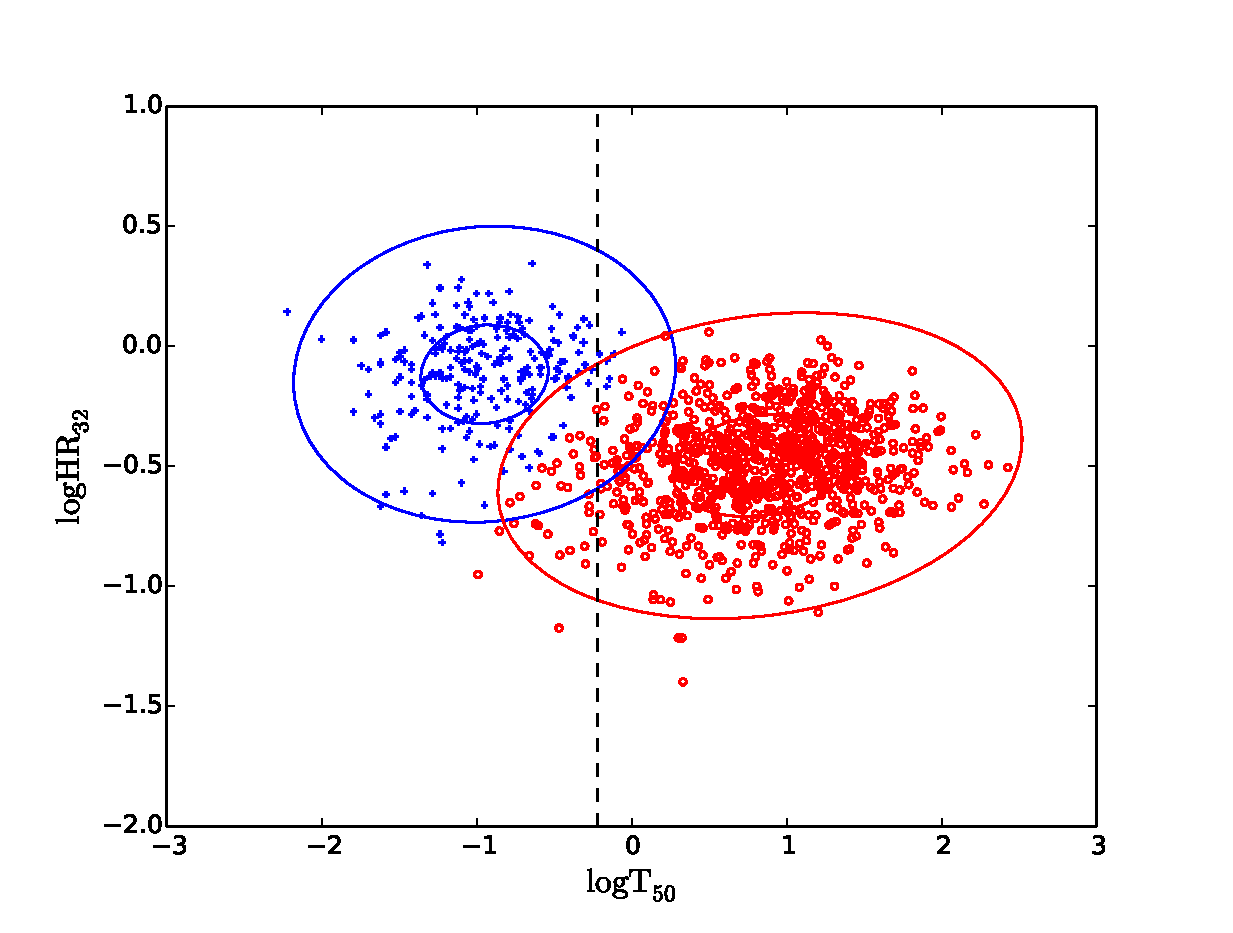
\includegraphics[width=1.0\textwidth]{list1143calHR_2} \\ а)}
  \end{minipage}
  \hfill
  \begin{minipage}[h]{0.5\textwidth}
    \center{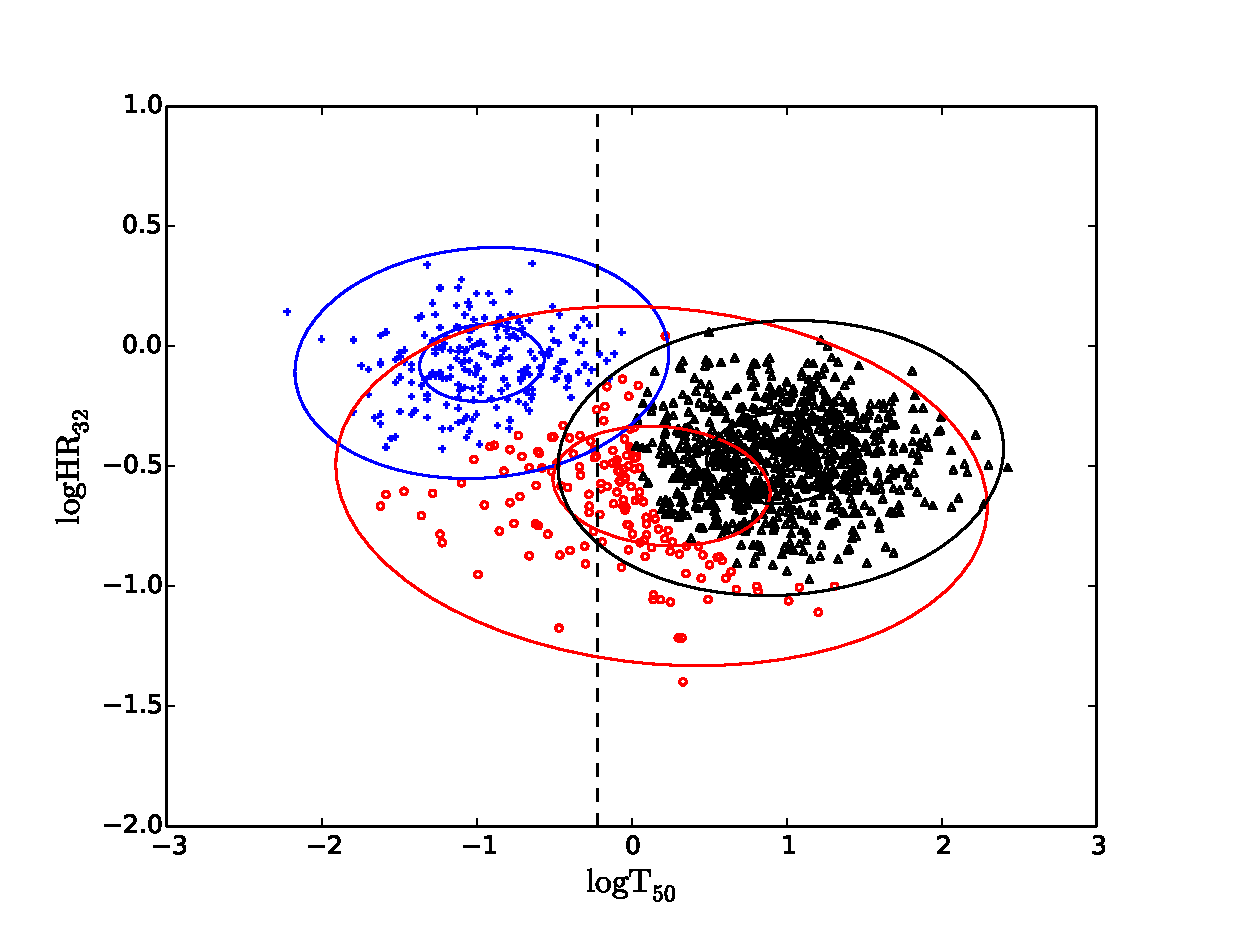
\includegraphics[width=1.0\textwidth]{list1143calHR_3} \\ б)}
  \end{minipage}
  \caption[Аппроксимация распределения $\log T_{50}$--$\log \mbox{HR}_{32}$.]
  {Аппроксимация распределения $\log T_{50}$--$\log \mbox{HR}_{32}$ 
  для 1143 ярких ($\rmn{S/N} \geq 10$) всплесков двумя~(a) и тремя~(б) гауссовыми компонентами. 
  Эллипсами для каждого распределения отмечены области $1\sigma$ и~$3\sigma$. 
  Пунктирная вертикальная линия~--- $T_{50} = 0.6$~с. Кресты~--- короткие/жесткие всплески, 
  круги~--- длинные/мягкие всплески, треугольники~--- промежуточные всплески. 
  Изображенное разделение сделано на основе $I_l$, но отличается от указанного в тексте для большей наглядности.
  Всплеск отнесён к кластеру $l$ если значение $I_l$ для этого кластера, 
  превышает значения для других кластеров.
  \label{img:HRvsT50}}
\end{figure}

\begin{figure} [h] 
  \center
  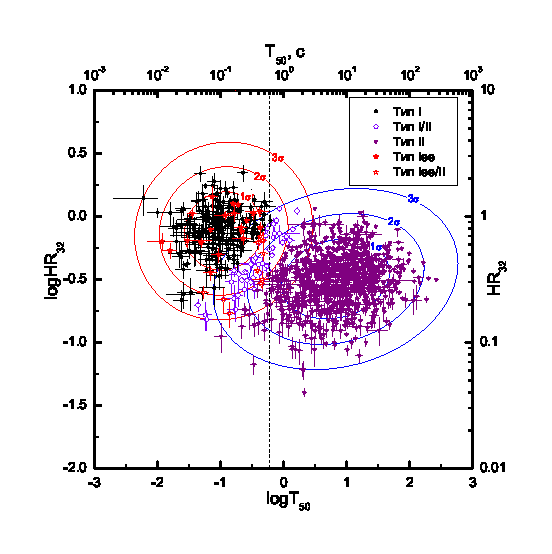
\includegraphics [width=0.75\textwidth] {gHRT50_Types_ru}
  \caption{Классификация 1143 ярких всплесков KW.
  Черные точки~--- Тип~I, круги~--- Тип~I/II, треугольники~--- Тип~II,
  см. описание методики классификации в тексте.
  } 
  \label{img:HRvsT50Types}  
\end{figure}

\begin{figure}[h]
  \begin{minipage}[h]{0.5\textwidth}
    \center{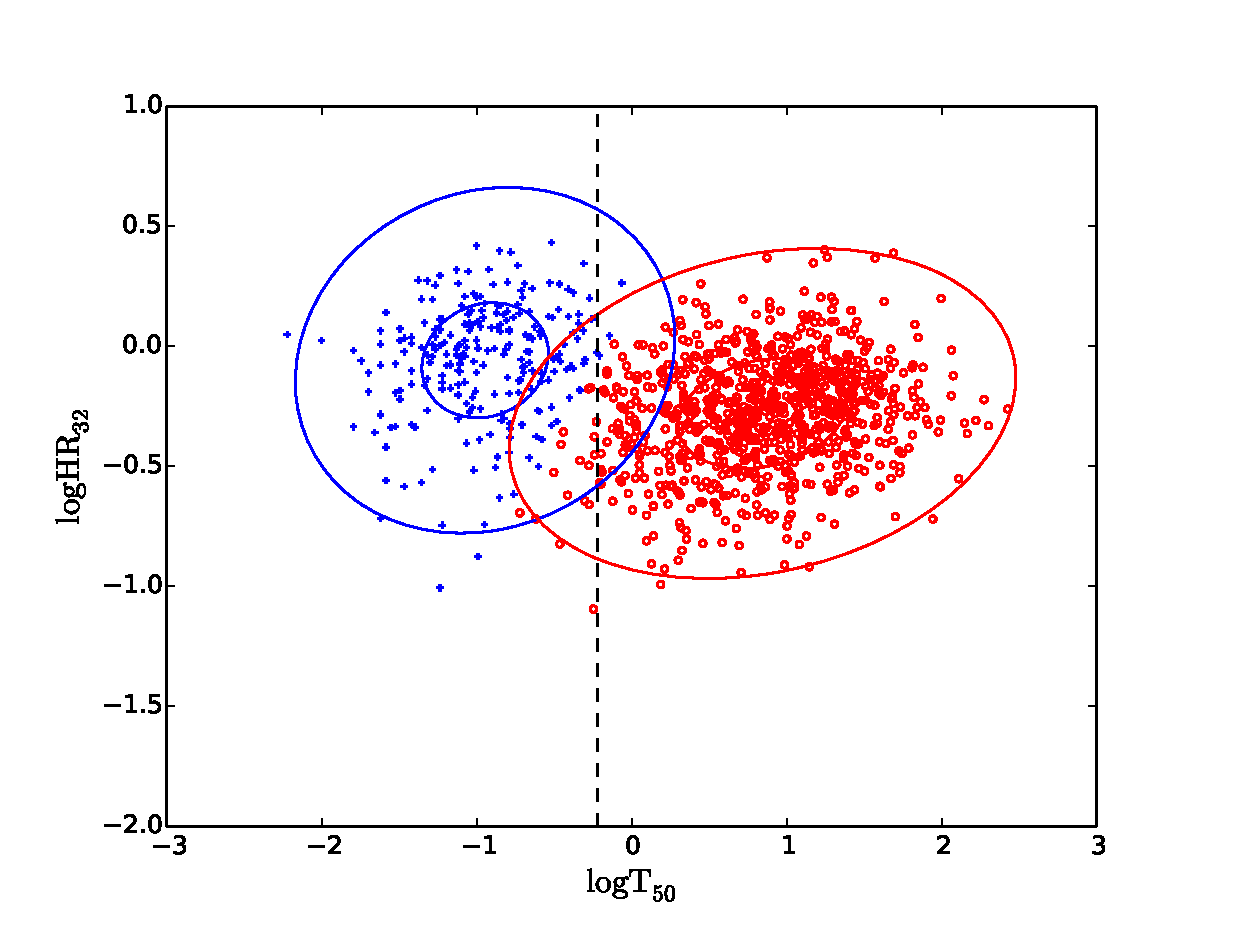
\includegraphics[width=1.0\textwidth]{list1104calHRpcr_2} \\ а)}
  \end{minipage}
  \hfill
  \begin{minipage}[h]{0.5\textwidth}
    \center{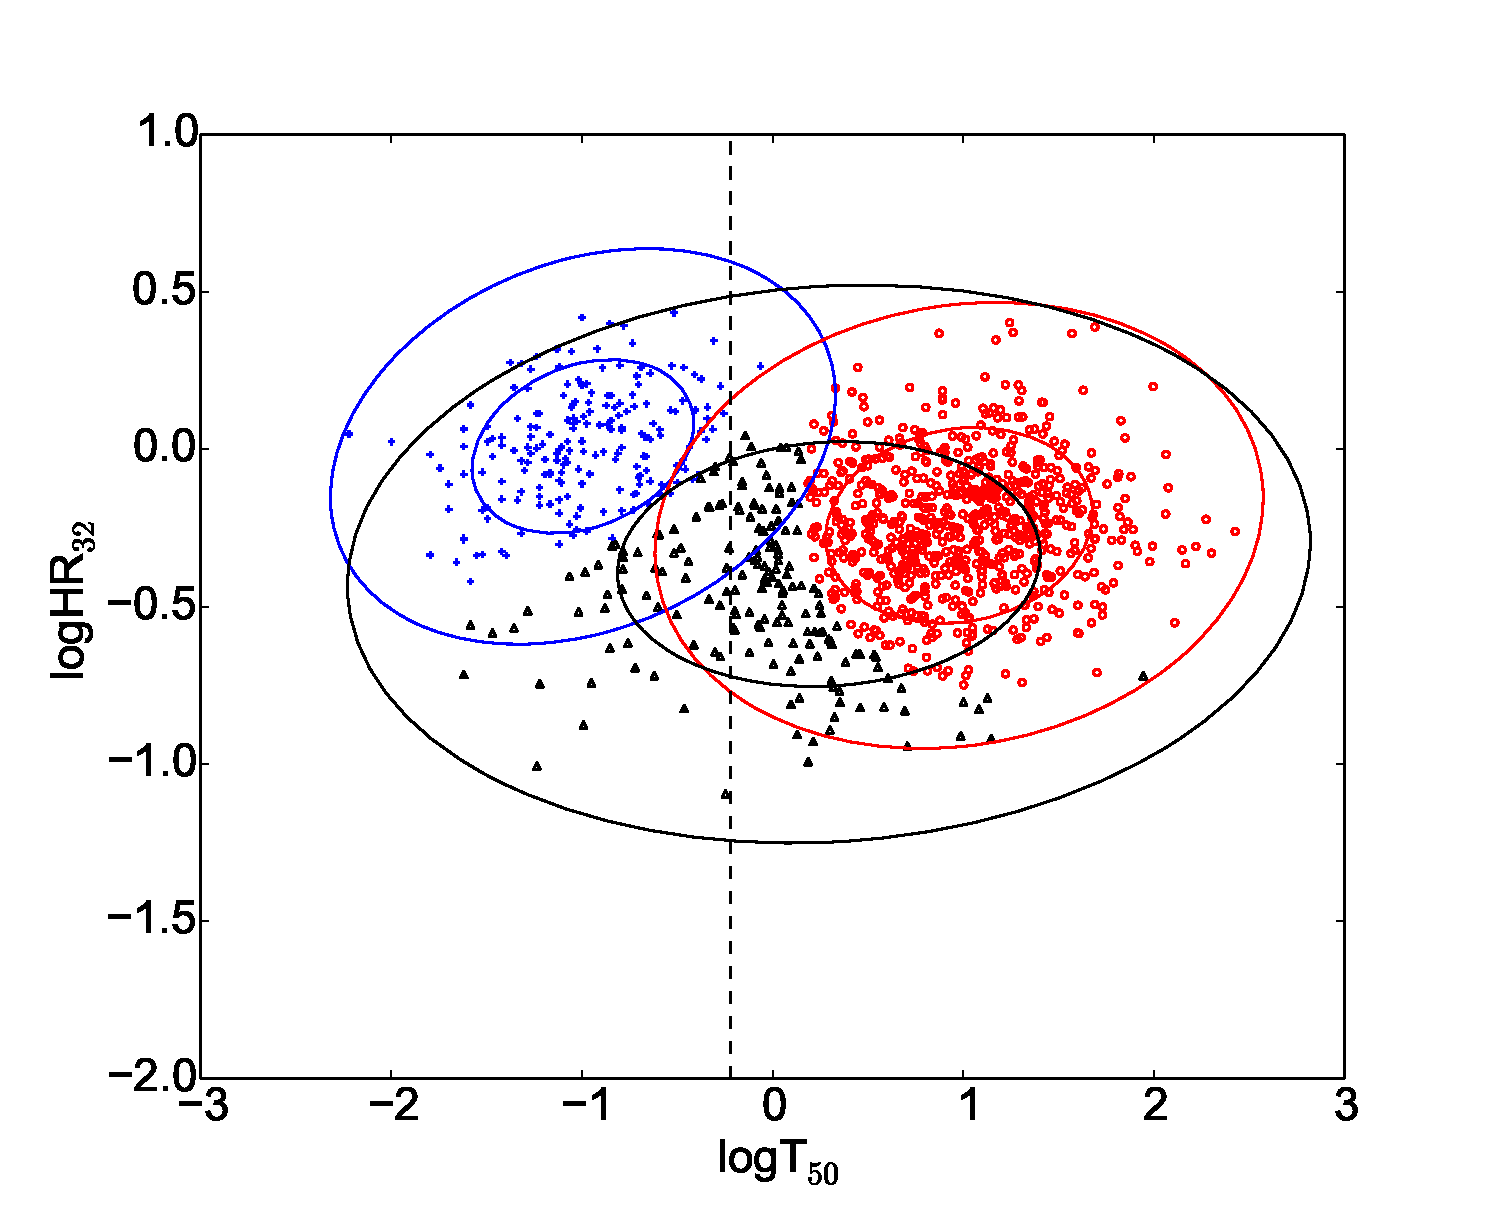
\includegraphics[width=1.0\textwidth]{list1104calHRpcr_3} \\ б)}
  \end{minipage}
  \caption[Аппроксимация распределения $\log T_{50}\textrm{--}\log \mbox{HR}_{32\rmn{pk}}$.]
  {Аппроксимация распределения $\log T_{50}\textrm{--}\log \mbox{HR}_{32\rmn{pk}}$ 
  для 1104 ярких всплесков ($\rmn{S/N} \geq 10$) двумя~(a) и тремя~(б) гауссовыми компонентами. 
  Эллипсами для каждого распределения отмечены области $1\sigma$ и~$3\sigma$. 
  Пунктирная вертикальная линия~--- $T_{50} = 0.6$~с. Кресты~--- короткие/жесткие всплески, 
  круги~--- длинные/мягкие всплески, треугольники~--- промежуточные всплески.
  Изображенное разделение сделано на основе $I_l$, но отличается от указанного в тексте для большей наглядности.
  Всплеск отнесён к кластеру $l$ если значение $I_l$ для этого кластера, 
  превышает значения для других кластеров.
  }
  \label{img:HRpkvsT50}  
\end{figure}

\FloatBarrier

\section{Спектральные задержки}\label{sec:Lags}
Одной из характеристик спектральной эволюции гамма-всплесков является спектральная задержка.
Она представляет собой количественную характеристику запаздывания излучения в 
мягком спектральном диапазоне по сравнению с более жестким~\citep[см., например,][Глава~3]{Minaev_PhD}.
Обзор моделей, описывающих появление спектральной задержки, смотри там же.
В данном разделе спектральная задержка используется исключительно в роли дополнительного 
параметра классификации гамма-всплесков, без обсуждения физической причины её возникновения. 

\subsection{Методика вычисления спектральных задержек для кривых блеска KW}
Для вычисления спектральных задержек всплесков KW использовался 
кросскорреляционный анализ временных историй~\citep{Band_1997ApJ, Norris_2000}. 
В этом методе задержка ($\tau_\rmn{lag}$) соответствует положению максимума 
кросс-корреляционной функции (ККФ) временных историй в различных каналах детектора.
Определение спектральной задержки между временными историями в двух диапазонах ($\tau_\rmn{lag}$) 
включало выбор разрешения временных историй, выбор интервала кросс-корреляции 
и вычисление $\tau_\rmn{lag}$ и её ошибки. 

Временное разрешение выбралось таким образом, чтобы для временных историй 
в обоих диапазонах бин с наибольшей скоростью счета имел отношение сигнал-шум~$\rmn{S/N} \geq 8$. 
Порог $\rmn{S/N} \geq 8$ был выбран произвольно, чтобы исключить из рассмотрения 
слабые всплески с большими ошибками $\tau_\rmn{lag}$. Возможные значения разрешения 
временной истории составляли от 4~мс до 1024~мс.
В качестве интервала кросс-корреляции брался наиболее широкий интервал, ограниченный
бинами, в которых было обнаружено превышение $5\sigma$ над фоном хотя бы в одном из каналов. 

Значение $\tau_\rmn{lag}$ и его ошибка определялись методом Монте-Карло на основе 
100 реализаций исходных кривых блеска. 
На каждой итерации генерировались искусственные временн\'{ы}е истории 
при помощи добавления пуассоновского шума к исходным данным.
На каждой итерации значения ККФ вычислялось аналогично формуле~(10) из~\citep{Band_1997ApJ}, 
ошибки ККФ вычислялись аналогично формуле~(5) из~\citep{Fenimore_1995}.
После построения ККФ производился поиск интервала, содержащего основной пик ККФ
при этом использовались только значения $>0.1$.  
После чего ККФ аппроксимировалась полиномом 4-й степени на выбранном интервале
и в качестве значения $\tau_\rmn{lag}$ брался максимум полинома.
Если $p$-значение аппроксимации (\textit{null hypothesis probability}) 
оказывалось меньше порогового значения 1\%, 
то из ККФ удалялись две крайние точки, и процедура повторялась до превышения порога. 
Если в результате уменьшения интервала аппроксимации число степеней свободы сокращалось до нуля,
то текущая итерация считалась неудачной. 
В случае, если итоговое число удачных итераций было больше $50$, то значение $\tau_\rmn{lag}$ 
вычислялось как среднее по всем удачным итерация, в качестве ошибки бралась дисперсия значений.
Иначе значение $\tau_\rmn{lag}$ считалось определенным ненадёжно и дальше не использовалось.
Примеры вычисления лага на одной из итераций представлены рис.~\ref{fig:lag_calculation}.

\begin{figure}[h]
  \center{\includegraphics[width=0.75\textwidth]{GRB20070512_T21972_lag_31}}
  \caption{Иллюстрация вычисления лага между кривыми блеска в G3 и G1 
   для короткого всплеска GRB20070512\_T21972 со значительной задержкой, $\tau_\rmn{lag}=277\pm16$~мс. 
  Вертикальные линии на нижней панели обозначают границы интервала кросс-корреляции. 
  Непрерывная линия на верхней панели показывает аппроксимацию ККФ полиномом 4-й степени. 
  Вертикальная пунктирная линия на верхней панели соответствует значению лага.
  \label{fig:lag_calculation}}  
\end{figure}

\subsection{Спектральные задержки коротких всплесков}
Спектральные задержки вычислялись между парами каналов G3--G1, G2--G1 и G3--G2, 
где $\tau_\rmn{lag}$ соответствует сдвигу временной истории в канале, указанном вторым
по отношению к каналу, указанному первым. Для коротких всплесков было получено
42, 66 и 158 задержек для пар каналов G3--G1, G2--G1 и G3--G2, соответственно.

На рис.~\ref{img:LagDistrs} представлены распределения коротких всплесков без EE и 
начальных импульсов коротких всплесков с EE по спектральным задержкам. 
Всплески Типа~I имеют, в основном, незначительные $\tau_\rmn{lag}\lesssim 25$~мс для 
пар каналов G3--G1 и G2--G1, при этом значительная часть всплесков типов~I/II и~II 
имеют задержки $\tau_\rmn{lag}\gtrsim 25$~мс для тех же пар каналов.

Среди коротких всплесков с продлённым излучением два события имеют существенные  % (ID=554, 1531)
спектральные задержки начального импульса в G3--G1 и были классифицированы Тип~Iee/II в предыдущем разделе. 
Таким образом, можно заключить, что значительная спектральная задержка подкрепляет классификацию 
на основе распределения на плоскости жёсткость-длительность.

\begin{figure}[h]
  \begin{minipage}[h]{0.5\textwidth}
    \center{\includegraphics[width=1.0\textwidth]{gDistLags} \\ а)}
  \end{minipage}
  \hfill
  \begin{minipage}[h]{0.5\textwidth}
    \center{\includegraphics[width=1.0\textwidth]{gDistLagsEE} \\ б)}
  \end{minipage}
  \caption{Распределение коротких всплесков без EE~(а) и начальных импульсов 
  всплесков с EE~(б) по спектральной задержке.
  На панели~(а), заполненная гистограмма~--- всплески Типа~I, заштрихованные 
  гистограммы~--- всплески Типа~I/II и~II.  На панели~(б), заполненная 
  гистограмма~--- всплески Типа~I, заштрихованные гистограммы~--- всплески Типа~Iee и~Iee/II.}
  \label{img:LagDistrs}  
\end{figure}

\FloatBarrier

\section{Сравнение классификаций на физические типы I и II всплесков KW 
с определенными красными смещениями}\label{sec:Phys_Classification}
Набор всплесков KW, зарегистрированных с ноября 1994~г. по июнь 2014~г., 
содержит 126 гамма-всплесков с измеренными красными смещениями~\citep{Tsvetkova_KW_GRBs_with_z}. 
Из них пять имеют сбои во временной истории, далее рассматривается набор из 121 всплесков. 
Указанный набор содержит 11 коротких и 110 длинных всплесков. 

Короткие всплески KW имеют красные смещения в диапазоне 0.1--1.0, длинные~--- 0.1--5.0.
Для $\sim 50$\% длинных и практически всех коротких всплесков из набора были 
определены физические типы на основе данных о послесвечении и родительских 
галактиках~\citep{Zhang_2009, Kann_2010ApJ, Kann_2011ApJ}.
При этом стоит выделить два всплеска. 
Длинный всплеск GRB~060614 относят к коротким всплескам с продлённым излучением~\citep{Gehrels_2006_Nature}. 
Однако, по данным KW его нельзя отнести к этому классу, так как на основе полной 
длительности $T_{50} = 49 \pm 5$~с, длительности его начального импульса 
$T_{50} = 2.7\pm 0.3$~с и жесткости этот всплеск относится к типу~II.
Всплеск GRB~040924 можно отнести к коротким всплескам на основе длительности $T_{50} = 0.34\pm0.06$~c, 
при этом он имеет значительную спектральную задержку, $120 \pm 30$~мс между каналами G2 и G1, 
и является достаточно мягким. По данным KW этот всплеск классифицируется как Тип~II, 
так же как и по данным многоволновых наблюдений~\citep{Zhang_2009}.

Было также проанализировано распределение жёсткость-длительность в системе 
отсчёта источника всплеска. При этом $T_{50}$ уменьшается в $1+z$~раз, а жёсткость 
вычислялась в каналах, чьи границы соответствуют номинальным умноженным на $1/(1+z)$. 
Распределения на плоскости $\log T_{50}$--$\log \mbox{HR}_{32}$ в системе отсчёта наблюдателя 
и собственной системе отсчёта представлены на рис.~\ref{img:T50HRzCorr}. 
Для сравнения распределений по жесткости и длительности всплесков типов I и II
в системе наблюдателя и собственной системе был использован тест Колмогорова-Смирнова для двух наборов. 
Вероятности (p-значения) того, что жесткости или длительности 
121-го всплеска являются выборкой из общего распределения малы ($<1$\%) 
как в случае системы наблюдателя, так и источника. Хотя в последнем случае
граница между типами становится размытой, рассмотренные распределения существенно отличаются,
что свидетельствует различие параметров коротких/жестких и длинных/мягких всплесков как 
в системе наблюдателя, так и системе источника всплеска. 

\begin{figure}[h]
  \begin{minipage}[h]{0.5\textwidth}
    \center{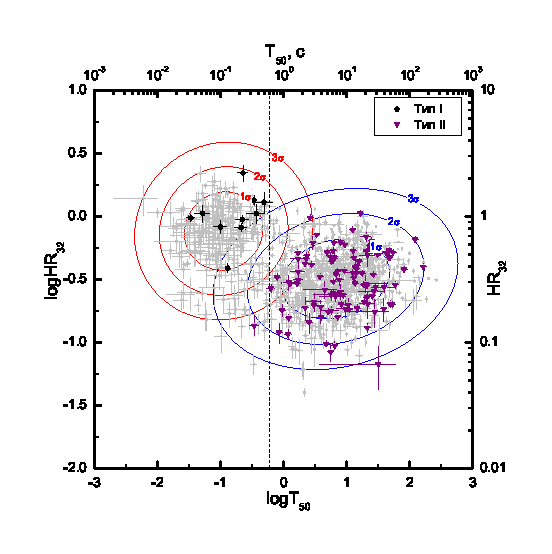
\includegraphics[width=1.0\textwidth]{gHRvsT50obs_ru} \\ а)}
  \end{minipage}
  \hfill
  \begin{minipage}[h]{0.5\textwidth}
    \center{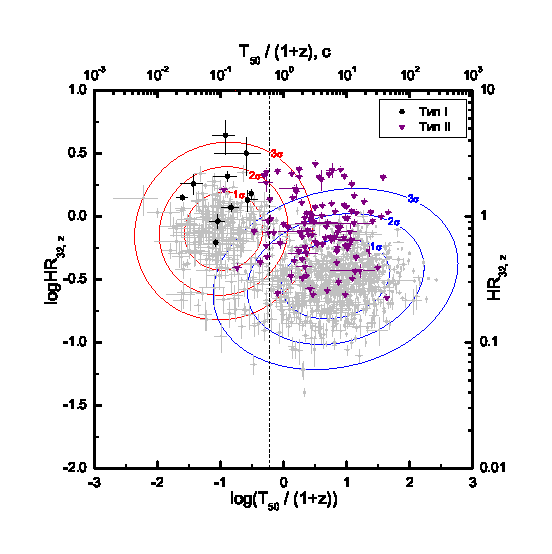
\includegraphics[width=1.0\textwidth]{gHRvsT50src_ru} \\ б)}
  \end{minipage}
  \caption{Распределение всплесков на плоскости $\log T_{50}$--$\log \rmn{HR}_{32}$ 
  в системе отсчёта наблюдателя~(а) и источника~(б), с поправкой на космологическое красное смещение. 
  Круги~--- всплески типа~I, треугольники~--- всплески типа~II, 
  серые точки~--- набор 1143 ярких всплесков.
  }
  \label{img:T50HRzCorr}  
\end{figure}

\section{Заключение} \label{sec:Conclision}
В данной главе описана методика классификации всплесков, зарегистрированных в эксперименте
Конус-Винд и получены следующие результаты:

\begin{enumerate}
\item Для набора 1834 всплесков KW были вычислены длительности $T_{50}$ и $T_{90}$, жесткости 
и спектральные задержки. Показано, что распределения 
всплесков по $T_{50}$ и $T_{90}$ хорошо аппроксимируются двумя логнормальными 
распределениями. Обнаружено, что параметры аппроксимации распределения $T_{50}$ 
более устойчивы к выбору порога поиска начала и конца всплеска, поэтому длительность 
$T_{50}$ более предпочтительна для классификации всплесков. В качестве границы между 
длинными и короткими всплесками была выбрана точка пересечения логнормальных компонент 
для порога значимости $5\sigma$, $T_{50} = 0.6$~с. 

\item Выбран набор коротких всплесков (без продлённого излучения), включающий 265 событий, 
что составляет 14\% от общего числа проанализированных всплесков. Для сравнения, 
доля коротких ($T_{90}<2$~с) всплесков в каталоге BATSE равна 24\%~\citep{Meegan_2001}, %(=500/2014)
в каталоге \textit{Fermi}-GBM 18\%~\citep{Paciesas_2012}, 
в каталоге \textit{Swift}-BAT 8\%~\citep{Sakamoto_2011ApJS}. 
Доля коротких всплесков, оцененная из площадей гауссовых компонент 
распределения $T_{50}$, равна 30\%. Соответствующая доля в наборе всплесков BATSE равна 32\%~\citep{Horvath_2002} 
и 8\% в наборе всплесков \textit{Swift}-BAT~\citep{Horvath_2008}.  

\item Обнаружен 31 всплеск, который можно классифицировать как короткий 
всплеск с продлённым излучением. Таким образом, доля всплесков с продлённым 
излучением среди коротких всплесков составляет 10\%. Соответствующая доля 
в выборке \textit{Swift}-BAT равна 20\%~\citep{Sakamoto_2011ApJS}. 
Спектральный анализ продлённого излучения представлен в главе~\ref{sGRB_spectral_catalog}.

\item Аппроксимация распределения всплесков на плоскости $\log T_{50}$--$\log \rmn{HR}_{32}$ 
набором гауссовых компонент показала наличие двух классов всплесков, коротких/жестких 
и длинных/мягких. При этом доля коротких/жестких всплесков, определённая на основе 
аппроксимации, составляет 21\%. По данным  BATSE доля коротких/жестких всплесков 
составляет 28\%~\citep{Horvath_2002}.  
Добавление третьей компоненты даёт значимое улучшения аппроксимации, однако эта 
компонента существенно перекрывается с компонентой, описывающей длинные всплески, 
и не представляет физического смысла. Дополнительный довод в пользу использования
только двух классов всплесков связан с тем, что для описания распределений 
по $T_{50}$ и $\rmn{HR}_{32}$ достаточно только двух компонент.
На основании полученной аппроксимации 7\% всплесков с $T_{50} < 0.6$~с относятся к типу~II.  (0.07=18/260)
При этом к типу~I относятся только всплески с $T_{50} < 0.6$~с 
(исключение составляет жесткий всплеск GRB20061006\_T31422 с пограничной  длительностью $T_{50} = 0.620\pm 0.049$~с, 
который не входит в набор коротких всплесков). Неопределенную классификацию (I/II) имеют 
около 4\% всплесков с длительностями $T_{50}$ от 0.04~с до 1.65~с.

На основании аппроксимации распределения $\log T_{50}$--$\log \rmn{HR}_{32}$ 
для 1143 всплесков, был классифицирован набор 265 коротких всплесков без продлённого излучения. 
Набор включает $\sim 70$\% всплесков Типа~I, $\sim 8$\% Типа~II и $\sim 12$\%
всплесков неопределённого типа (I или~II). Доля коротких всплесков с продлённым 
излучением составляет $\sim 10$\%.
Среди начальных импульсов всплесков, отнесённых на основе морфологии временной 
истории к коротким всплескам с продлённым излучением, 21 (68\%) классифицированы как Тип~I 
7 как неопределённый тип (I/II) и 3 как Тип~II.
 
\item Анализ спектральных задержек коротких всплесков показал, что большинство коротких всплесков 
Типа~I имеют незначительную по абсолютному значению спектральную задержку $\tau_\rmn{lag} \lesssim 25$~мс, 
в то же время значительная доля всплески типов~II и I/II имеет $\tau_\rmn{lag} > 25$~мс. 
Два всплеска с продленным излучением имеют задержку начального импульса $> 100$~мс
и были классифицированы как тип~II, что свидетельствует о том, что
эти всплески относятся к популяции длинных всплесков.  

\item Сравнение классификаций на физические типы~I и~II с классификацией на основе 
длительности, жесткости и спектральной задержки подтвердило, что всплески Типа~I 
относятся к коротким/жестким всплескам с малой спектральной задержкой, а всплески 
Типа~II, в основном,~--- длинные мягкие с заметной спектральной задержкой. 
Сравнение распределений $\log T_{50}$--$\log \rmn{HR}_{32}$ в системе отсчёта наблюдателя 
и в собственной системе отсчёта показывает, что различие в жесткости и длительности
всплесков типа~I и~II становится менее значимым, но сохраняется.
\end{enumerate}

Для дальнейшего анализа выбран полный набор 296 коротких всплесков. 
Различия между короткими всплесками разных типов будут подробно исследованы на
основе спектрального анализа всплесков в главе~\ref{sGRB_spectral_catalog}.

По материалам Главы~\ref{KW_GRB_classification} на защиту выносится следующее положение:
\begin{itemize}
\item Метод классификации гамма-всплесков по данным эксперимента Конус-Винд на основе
    длительности и жесткости излучения всплеска, а также величин спектральных задержек.
\end{itemize}

\clearpage